\section{Progrès réalisé}

\subsection{I.A. - Intelligence Artificielle}
\setlength{\parindent}{5ex}
Pour implémenter une intelligence artificielle, nous avons testé divers algorithmes de ''pathfinding'' dans un grand nombre de scènes comprenant des obstacles afin de pouvoir implémenter dans notre jeu une entité antagoniste qui suivra le joueur.

\begin{figure}[H]
\centering
\begin{minipage}{.5\textwidth}
  \centering
  \centerline{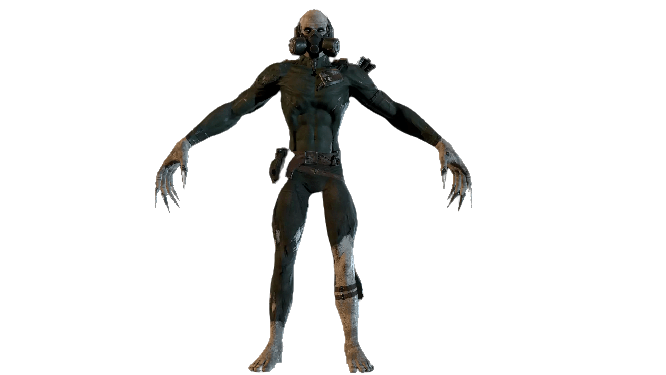
\includegraphics[width=1\linewidth]{img/assets/sterven.png}}
  \captionof{figure}{\emph{Entité}}
  \label{fig:méchant}
\end{minipage}%
\end{figure}

Notre entité utilisera le pathfinding pour déterminer, dès lors que le joueur rentrera dans son champ d'action, un chemin à suivre pour atteindre le joueur et l'attaquer.

\begin{figure}[H]
\centering
\begin{minipage}{.5\textwidth}
  \centering
  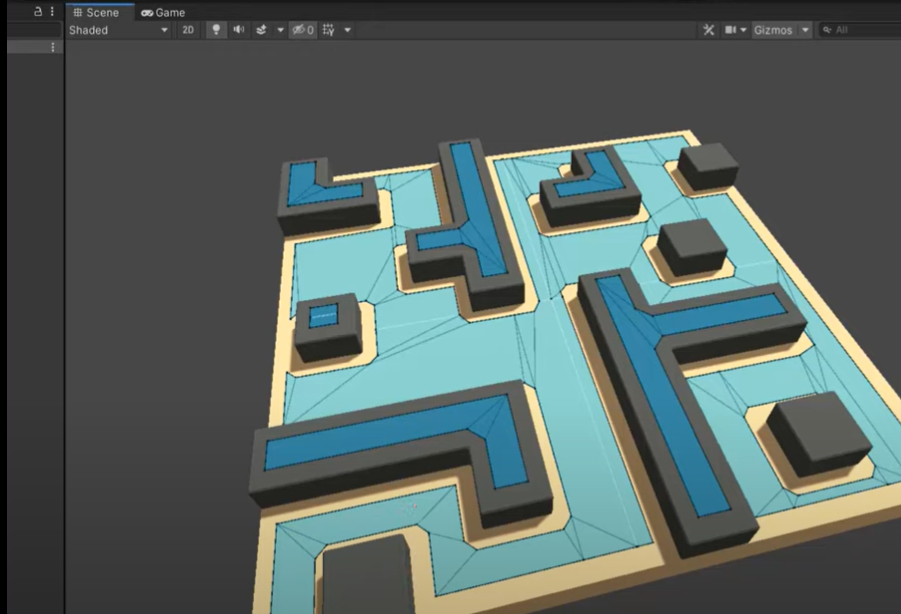
\includegraphics[width=.7\linewidth]{img/navmesh.PNG}
  \captionof{figure}{\emph{NavMesh : Tous les endroits possibles au déplacement de l'entité}}
  \label{fig:navmesh}
\end{minipage}%
\begin{minipage}{.5\textwidth}
  \centering
  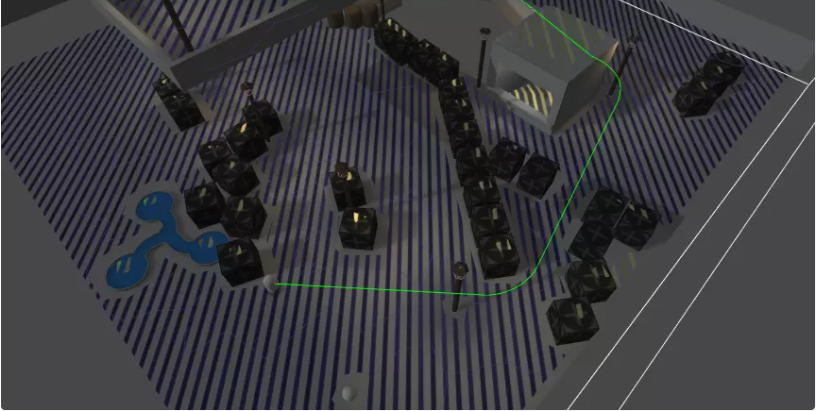
\includegraphics[width=.7\linewidth]{img/path.png}
  \captionof{figure}{\emph{Pathfinding}}
  \label{fig:pathfinding}
\end{minipage}
\end{figure}

\vfill
\noindent\makebox[\linewidth]{\rule{.8\paperwidth}{.6pt}}\\[0.2cm]
EPITA Toulouse - Projet S2 - 2022 \hfill Nyctalopia - gameHUB
\noindent\makebox[\linewidth]{\rule{.8\paperwidth}{.6pt}}

\newpage

\subsection{Audio et Effets Sonores}
\setlength{\parindent}{5ex}
Pour l’audio, la cinématique principale et le menu d’accueil du jeu comptent déjà avec ses propres musiques, libres de droits et utilisables pour usage commercial, qui représentent bien l’aspect mystérieux et effrayant de notre jeu d’horreur.



Les effets sonores du menu d’accueil ont déjà été mis en place et les effets extradiégétiques trouvables dans le jeu ont déjà été sélectionnés (ramassage d’objets, interaction quelconque).

Nous continuons d’effectuer des recherches concernant les effets sonores liés aux différents matériaux du jeu lorsque les joueurs y marchent dessus. Cependant, les effets sonores gratuits seront très accessibles grâce aux bibliothèques d’effets sonores gratuits \emph{Zapsplat} ou \emph{Freesound} auxquelles on a déjà jeté un coup d’œil. 


\subsection{Gameplay}
\setlength{\parindent}{5ex}
Lors de la première soutenance nous avons ajouté des scripts permettant au joueur de se déplacer, de pouvoir s’accroupir et de pouvoir diriger la caméra.
\newline
Depuis nous avons ajouté deux scripts principaux à notre projet :
\begin{description}
  \item[\emph{PlayerStatut -}] une classe permettant de stocker l’avancée du joueur dans sa partie. Ce script permet de tenir à jour la réussite des différents puzzles et l’ouverture de différentes portes du jeu à travers la récupération des divers objets nécessaires à leur réussite ou leur ouverture. Ce script gardera aussi en mémoire les coordonnées du dernier point de sauvegarde utilisé pour y placer le joueur lors de sa prochaine mort ou du prochain lancement de la partie.
  Pour réaliser se script, nous avons eu besoin de créer deux autres classes
  \begin{description}
    \item[$\bullet$ \emph{Item} -] qui contiendra l’identifiant de l’objet
    \item[$\bullet$ \emph{Environnement} -] qui contiendra l’identifiant des portes et énigmes résolues par le joueur
\end{description}
\emph{PlayerStatut} stocke ces différents \emph{Items} et \emph{Environnement} dans des listes.
Lors de l’ouverture d’une porte fermée on vérifiera si l’\emph{Items} correspondant à la clé est bien dans le \emph{PlayerStatut} du joueur et on ajoutera cette porte à une liste d’\emph{Environnement}. Lors du prochain lancement de la partie, le jeu reprendra au même stade grâce aux coordonnées du point de sauvegarde et au suivi des différentes ouvertures.
De plus une classe \emph{Translate} comprend tous les équivalent nom/identifiant des objets, des portes, des puzzles pour faciliter la compréhension du code en plus des coordonnées des points de sauvegarde.
Pour les points de sauvegarde : chaque point est lié à ses coordonnées dans le jeu.
\end{description}

\vfill
\noindent\makebox[\linewidth]{\rule{.8\paperwidth}{.6pt}}\\[0.2cm]
EPITA Toulouse - Projet S2 - 2022 \hfill Nyctalopia - gameHUB
\noindent\makebox[\linewidth]{\rule{.8\paperwidth}{.6pt}}

\begin{description}
  \item[\emph{SaveData -}] un script qui sera par la suite lié aux bornes de sauvegarde dissimilées à des endroits prédéfinis dans le jeu. Ce script permet de sauvegarder des données dans le répertoire crée lors de l’installation du jeu grâce à la méthode \emph{Application.persistentPath} mise à disposition par Unity. Les données sauvegardées sont contenues dans le \emph{PlayerStatut} (mentionné ci-dessus), et seront stockées dans le format JSON (1) et chiffrées grâce au chiffrage XOR (XOR Cipher) (2), empêchant ainsi le joueur de tricher en modifiant sa sauvegarde. Pour des raisons pratiques, lors des tests et des présentations, un mode développeur sera disponible permettant de modifier la sauvegarde et avancer à l’état souhaité du jeu.
\end{description}

\begin{description}
    \item[(1) :] Le format JSON (JavaScript Object Notation) est un format couramment utilisé pour représenter de l’information structurée sous forme de texte, il est facilement lisible par des humains (malgré le manque d’espaces nécessaire pour alléger le fichier).
    \begin{figure}[H]
        \centering
        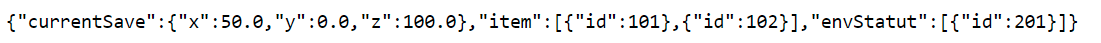
\includegraphics[width=18cm]{img/gameplay/JSONRaw.PNG}
        \caption{ Fichier JSON}
        \label{fig:JSONraw}
    \end{figure}
    \item[(2) :] Le chiffrage XOR utilise l’opérateur binaire XOR (OU-exclusif), voici sa table de vérité:
    \newline
    \begin{figure}[H]
        \centering
        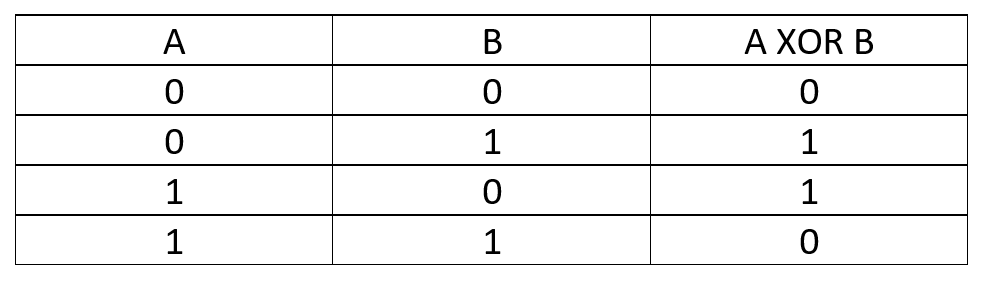
\includegraphics[width=10cm]{img/gameplay/XORtable.PNG}
        \caption{ Table de vérité OU-exclusif}
        \label{fig:XORtable}
    \end{figure}
\end{description}
\par
Lors du chiffrage nous allons passer à travers une porte logique XOR chaque lettre de nôtre chaîne de caractère avec la lettre au même indice, le tout modulo la longueur de notre clé, et ainsi reconstruire une chaîne de caractères chiffrée, de même longueur mais inintelligible.
Lors du déchiffrement nous allons effectuer les mêmes actions mais avec la chaîne de caractères chiffrée à la place de celle en claire.
Pour passer deux lettres à travers la porte XOR on passe en réalité les représentations binaires des codes ASCII (American Standard Code for Information Interchange) de ces lettres, le résultat sera donc une représentation binaire convertie en nombre et retranscrite grâce à la table ASCII.
Exemple : 
Dans cet exemple on souhaite chiffrer le mot ''MESSAGE'' avec la clé ''CLE'' :

\vfill
\noindent\makebox[\linewidth]{\rule{.8\paperwidth}{.6pt}}\\[0.2cm]
EPITA Toulouse - Projet S2 - 2022 \hfill Nyctalopia - gameHUB
\noindent\makebox[\linewidth]{\rule{.8\paperwidth}{.6pt}}

    \begin{figure}[H]
        \centering
        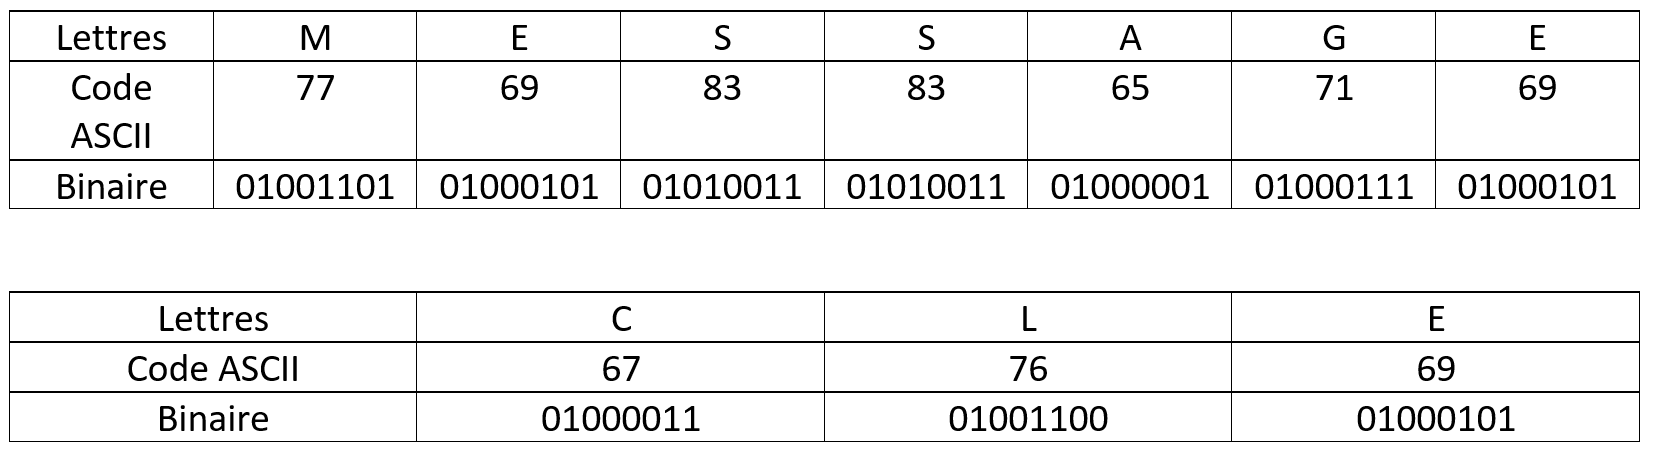
\includegraphics[width=15cm]{img/gameplay/clemsgtranscript.PNG}
        \caption{ Conversion des lettres en binaire}
        \label{fig:transciption}
    \end{figure}
    
Le chiffrement XOR va donc correspondre à ceci :
 \newline
    \begin{figure}[H]
        \centering
        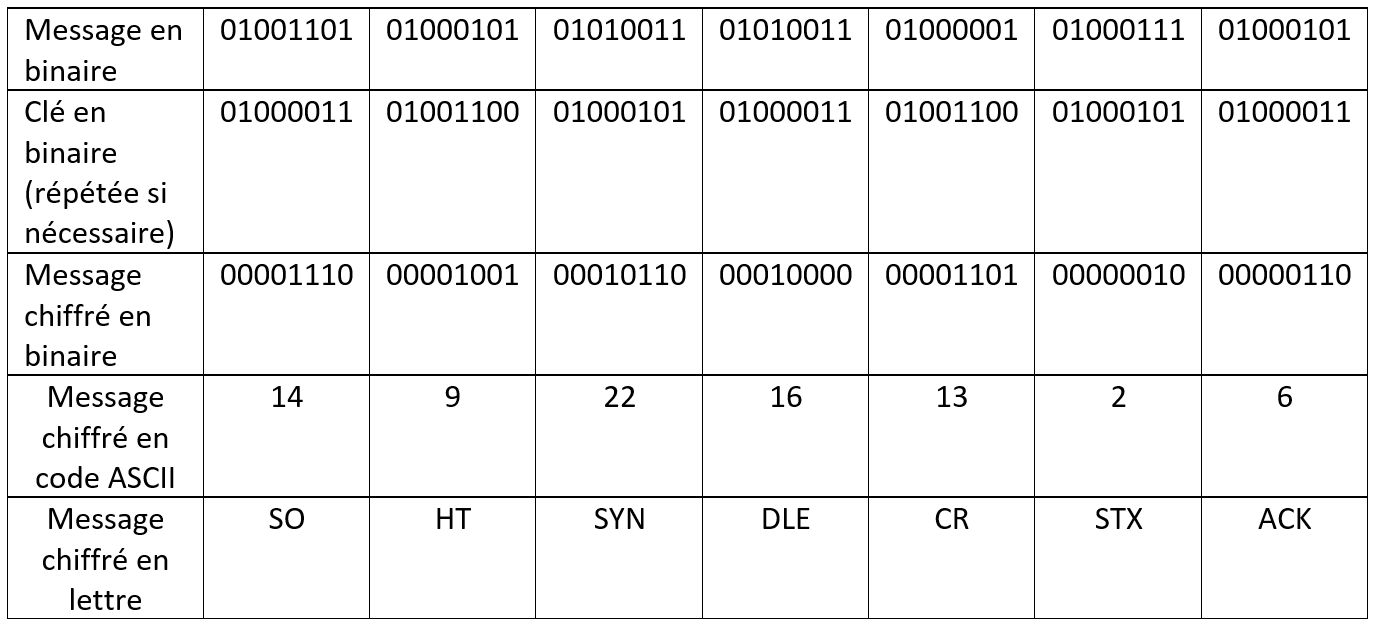
\includegraphics[width=17cm]{img/gameplay/Xorencryot.PNG}
        \caption{ Conversion des lettres en binaire}
        \label{fig:XORencryption}
    \end{figure}

Dans cet exemple le message chiffré est composé uniquement de caractères ASCII non imprimables, de caractères de contrôle, utilisés pour contrôler certains périphériques ou donner des indications sur le format du document.
\newline
Le chiffrement XOR est basique et le message chiffré peut être facilement décrypté si la clé est trop petite par rapport à la taille du message grâce à une analyse fréquentielle ou dans ce cas d’utilisation (sauvegarde) par une attaque à texte clair connue comme le joueur connaît par exemple les noms des objets.
\newline
Nous avons choisi de créer une clé de 50 caractères choisis aléatoirement parmi les caractères dite imprimable de la table ASCII.

\vfill
\noindent\makebox[\linewidth]{\rule{.8\paperwidth}{.6pt}}\\[0.2cm]
EPITA Toulouse - Projet S2 - 2022 \hfill Nyctalopia - gameHUB
\noindent\makebox[\linewidth]{\rule{.8\paperwidth}{.6pt}}

Il est donc ici préférable de se référer aux objets par des nombres plutôt que des noms, nous choisissons de représenter les objets, les portes et énigmes réussit par des identifiants.
Pour un souci de lisibilité nous avons aussi ajouté un dictionnaire liant les identifiants des objets, portes et énigmes à leurs noms.
\newline
De plus, pour l’instant, la clé de chiffrement est unique pour toutes les sauvegardes et tous les joueurs mais il peut être intéressant d’en générer une nouvelle aléatoirement à chaque création d’une nouvelle partie en retranscrivant ce code en C\#.


Nous avons aussi commencé les recherches et l’implémentation de la touche ''utiliser'' assignée par défaut à la touche ''E''. Nous utiliserons le système de \emph{RayCast} (qui peut être traduit par ‘’lancé de rayon’’) et le système \emph{Event} proposé par Unity et découper ce système en deux scripts distincts: \emph{Interactor} et \emph{Interactable}. Ils seront respectivement liés au joueur et aux objets que l’on veut interactifs tels que les bornes de sauvegarde, les puzzles, les clés à récupérer, les portes…
\newline
\begin{description}
    \item[\emph{Interactor} -] Ce script sera composé d’un RayCast dont la portée représentera la portée d’action du joueur dans le jeu et vérifiera si l’objet pointé par le joueur est étiqueté comme interactif et s’il n’y a pas d’objets entre celui-ci et le joueur rendant l’action impossible tel qu'un mur par exemple. Ensuite nous vérifierons si le joueur appuie bien sur la touche d’action.
    \item[\emph{Interactable} -] Ce script comportera l’évènement associé à l’objet interactif : récupération d’une clé (disparition de celle-ci et son ajout dans le \emph{PlayerStatut}), ouverture d’une porte (vérification que la clé est bien en possession du joueur, si oui, ouverture de la porte).
\end{description}
\par
Nous pourrons aussi par la suite implémenter un curseur changeant de forme si le joueur pointe et est en assez proche d’un objet interactif (passage d’une croix à une main par exemple).
\par
Concernant le changement des touches, nous avons décidé pour l’instant de laisser le choix au joueur entre deux configurations ''AZERTY'' et ''QWERTY'' qui est plus rapide à implémenter. La personnalisation des touches prend tu temps à implémenter et n’est pas vitale, nous avons donc décidé de repousser son implémentation à plus tard.


\vfill
\noindent\makebox[\linewidth]{\rule{.8\paperwidth}{.6pt}}\\[0.2cm]
EPITA Toulouse - Projet S2 - 2022 \hfill Nyctalopia - gameHUB
\noindent\makebox[\linewidth]{\rule{.8\paperwidth}{.6pt}}


\subsection{Communication}
\setlength{\parindent}{5ex}

La police d'écriture temporaire du logo du jeu Nyctalopia (actuellement : ``\emph{Venom}'') a été remplacée par la police ``\emph{October} Crow''.

\begin{figure}[H]
\centering
\begin{minipage}{.5\textwidth}
  \centering
  \centerline{
\includegraphics[width=1.5\linewidth]{img/font.png}}
  \captionof{figure}{\emph{Police d'écriture choisie pour Nyctalopia}}
  \label{fig:octobercrowfont}
\end{minipage}%
\end{figure}

\vfill
\noindent\makebox[\linewidth]{\rule{.8\paperwidth}{.6pt}}\\[0.2cm]
EPITA Toulouse - Projet S2 - 2022 \hfill Nyctalopia - gameHUB
\noindent\makebox[\linewidth]{\rule{.8\paperwidth}{.6pt}}

\subsection{Graphismes, Modèles et Terrain}
\setlength{\parindent}{5ex}
L'histoire du jeu se basera sous forme de chapitres, le premier est le Chapitre 0, c'est une cinématique d'une minute trente secondes, où le joueur est immédiatement accueilli par un accident de voiture.

\begin{figure}[H]
\centering
\begin{minipage}{.5\textwidth}
  \centering
  \centerline{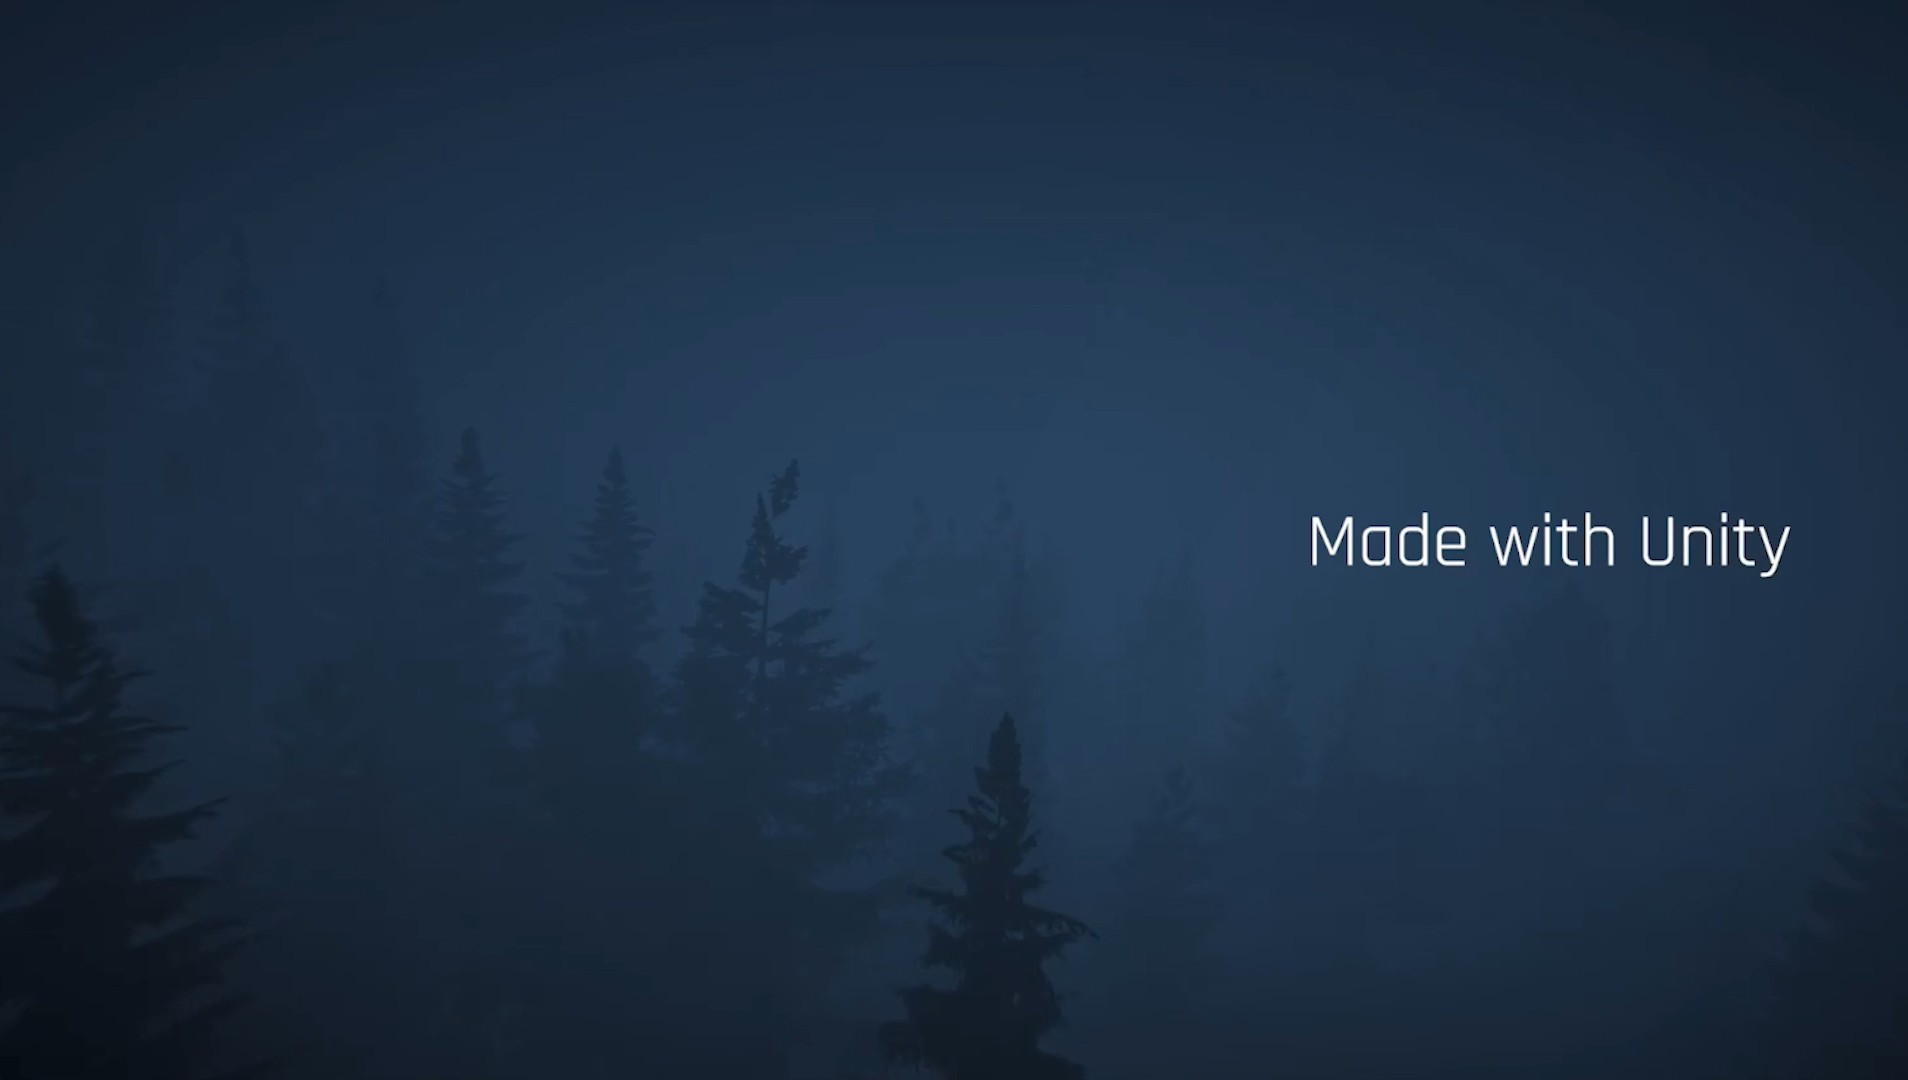
\includegraphics[width=1\linewidth]{img/cine.png}}
  \captionof{figure}{\emph{Chapitre 0}}
  \label{fig:cinematique}
\end{minipage}%
\end{figure}

Une grande variété de modèles 3D d’arbres, arbustes et herbe ont déjà été sélectionnés et utilisés dans le jeu pour couvrir ce terrain et créer une forêt riche et variée. La plupart de ces modèles de végétation proviennent de la bibliothèque de modèles 3D \emph{Quixel’s Megascans} et du site officiel de modèles Unity \emph{Unity Asset Store}. Plusieurs modifications et conversions ont été nécessaires pour les rendre compatibles avec notre projet qui est basé sur le système de rendu HDRP (\emph{High-Definition Render Pipeline}) qui offre des résultats graphiques plus attractifs.
\newline

Nous aurons ensuite une partie qui se déroulera dans la forêt (Chapitres 1 et 2) avec des énigmes et puzzles à résoudre tout au long de ces chapitres.

\begin{figure}[H]
\centering
\begin{minipage}{.5\textwidth}
  \centering
  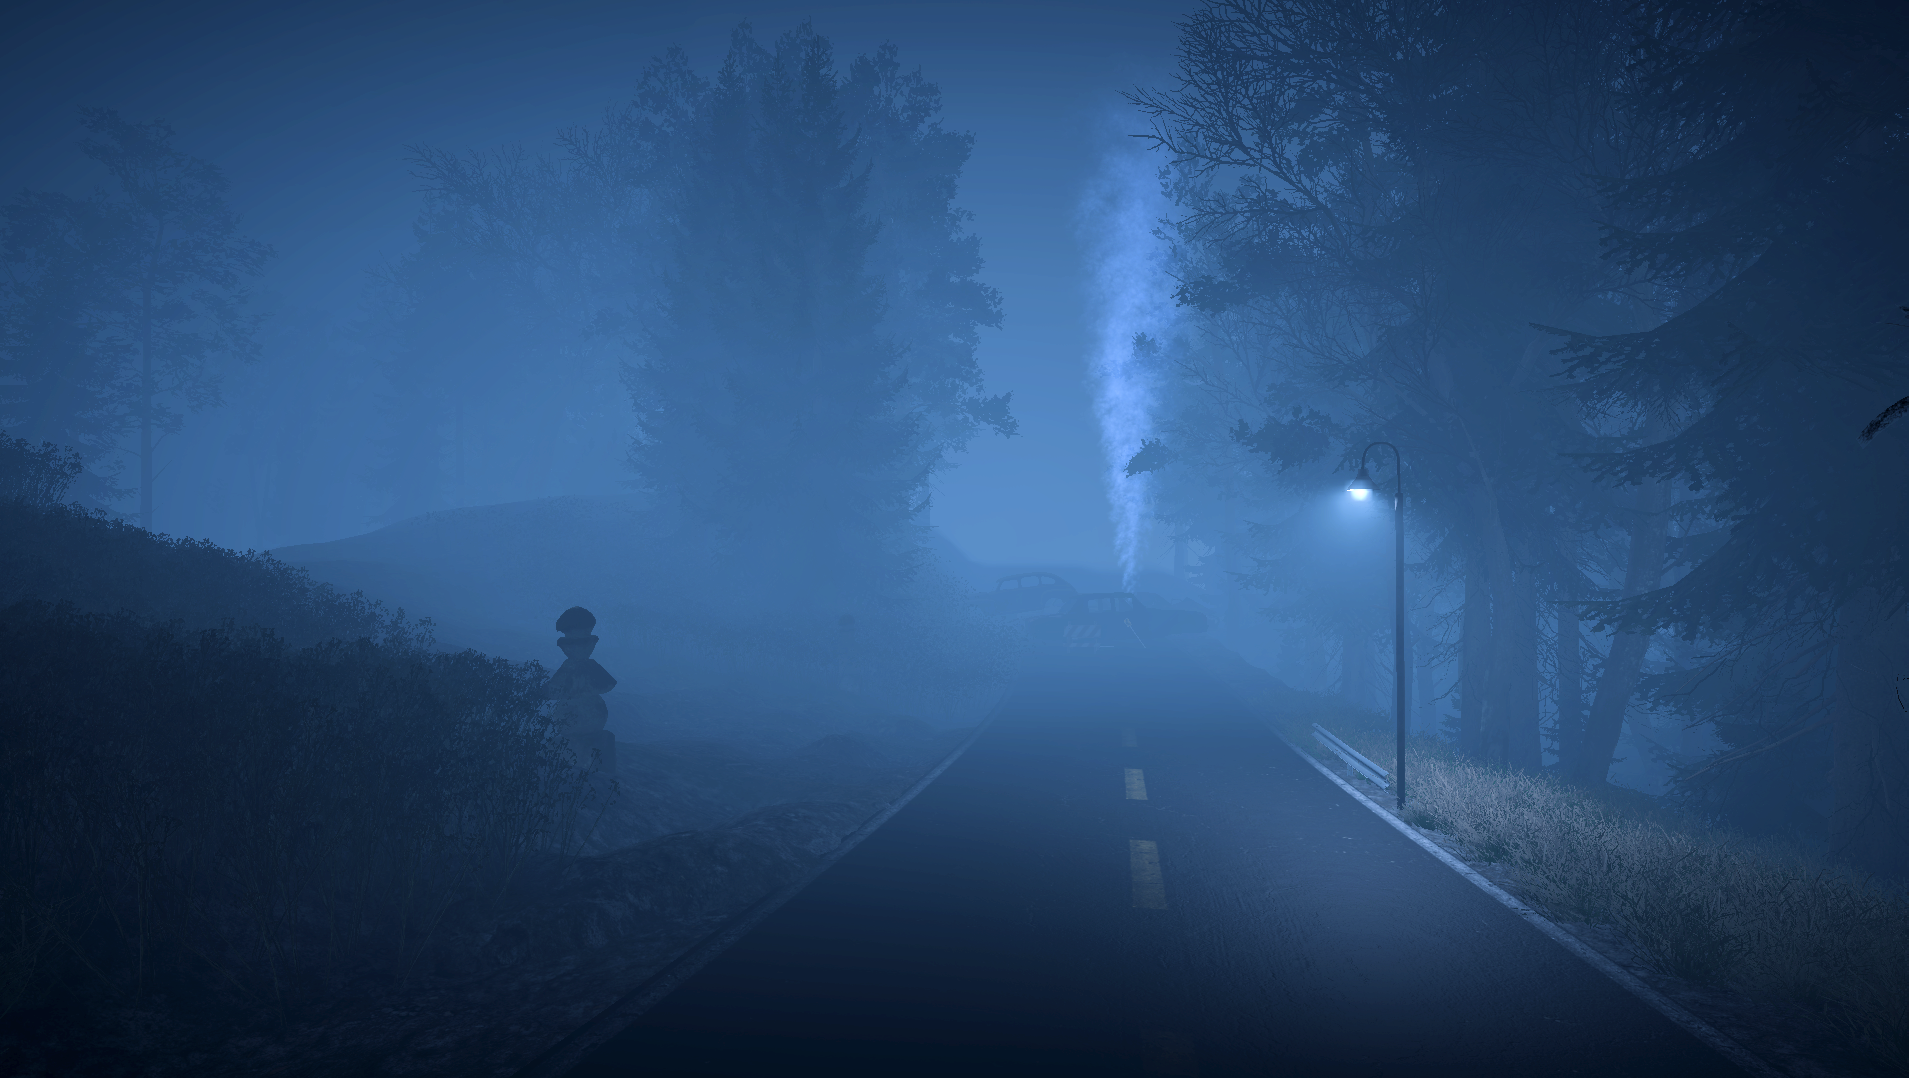
\includegraphics[width=.7\linewidth]{img/uwufolder/spawn.png}
  \captionof{figure}{\emph{Représentation du Chapitre 1}}
  \label{fig:égouts1}
\end{minipage}%
\begin{minipage}{.5\textwidth}
  \centering
  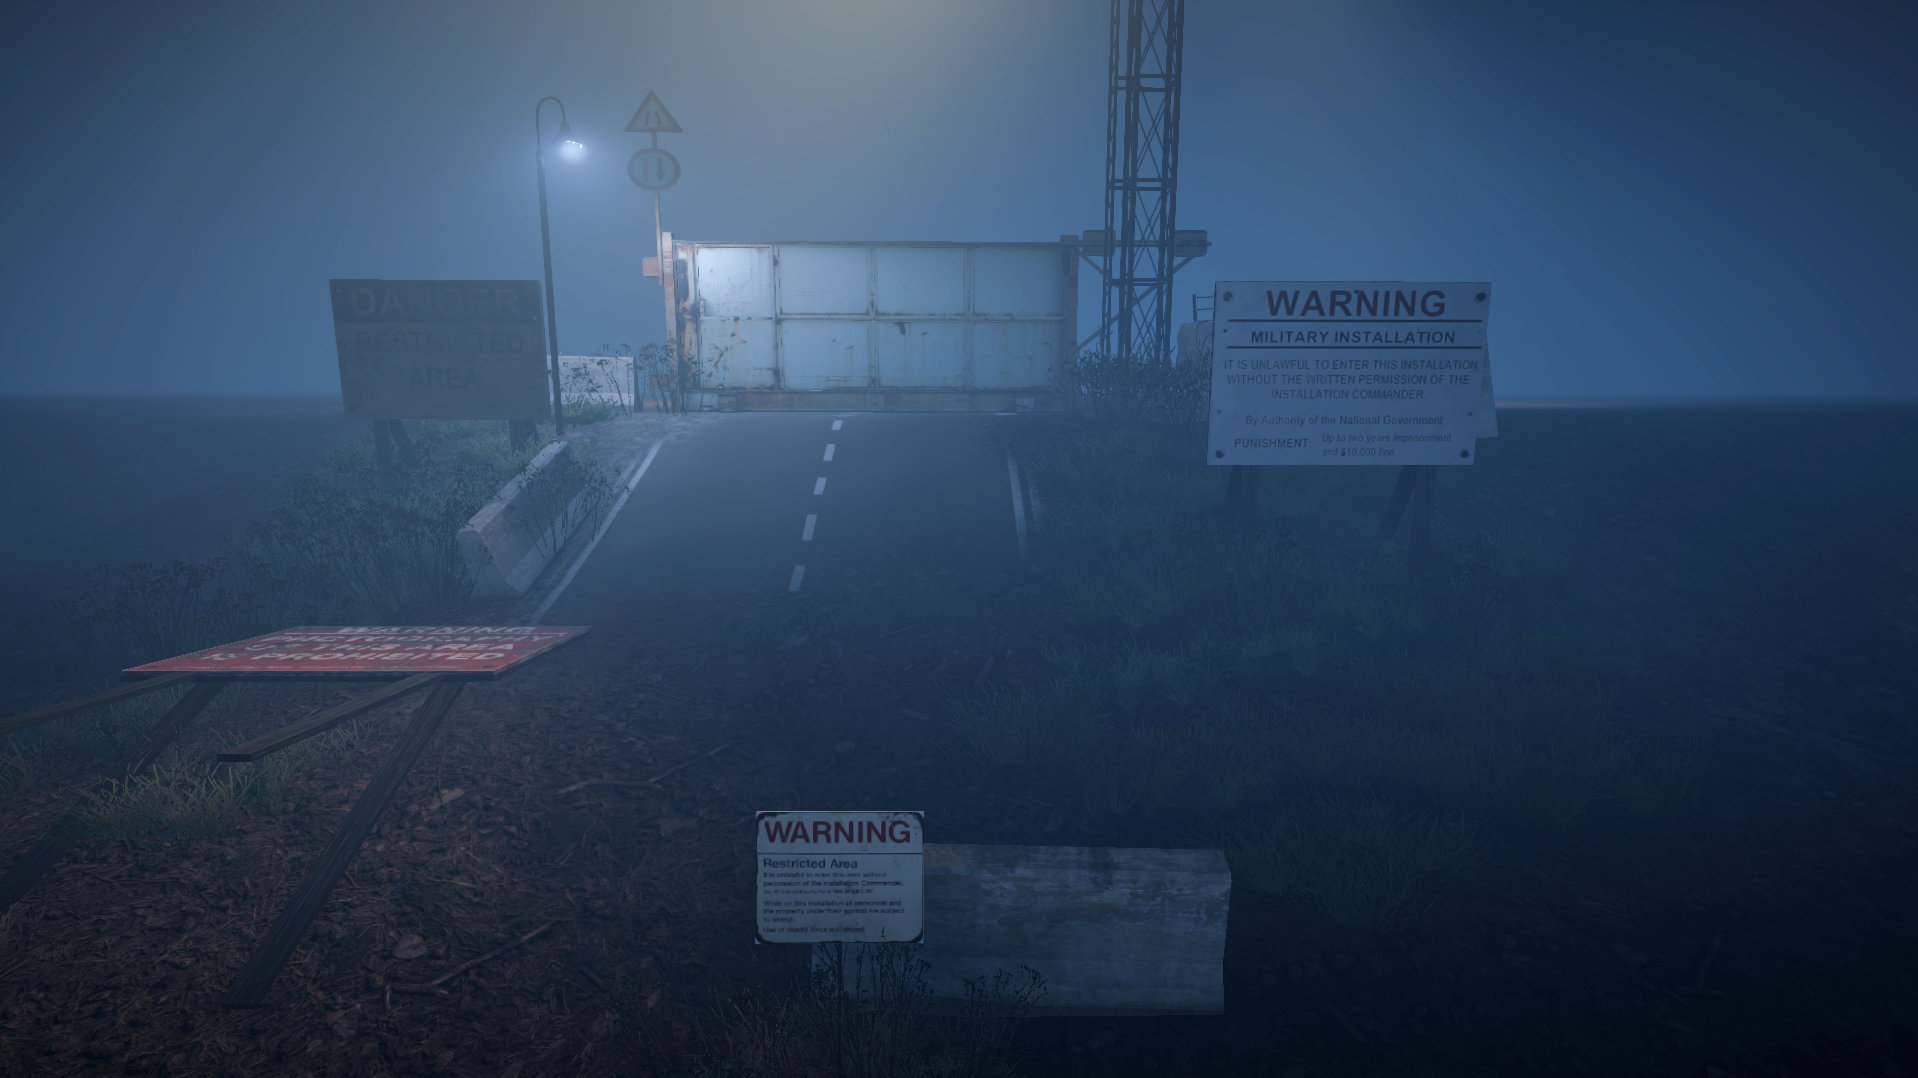
\includegraphics[width=.7\linewidth]{img/uwufolder/military.png}
  \captionof{figure}{\emph{Représentation du Chapitre 2}}
  \label{fig:égouts2}
\end{minipage}
\end{figure}





Enfin un troisième chapitre est déjà en cours de production, qui se déroulera, dans des souterrains. Dans ce nouvel espace jouable, le joueur devra, dans le noir et grâce à une lampe torche, trouver un moyen de s'échapper le tout en évitant l'entité antagoniste qui sera enfermée avec lui et qui le suivra avec un algorithme de \emph{pathfinding}.

\vfill
\noindent\makebox[\linewidth]{\rule{.8\paperwidth}{.6pt}}\\[0.2cm]
EPITA Toulouse - Projet S2 - 2022 \hfill Nyctalopia - gameHUB
\noindent\makebox[\linewidth]{\rule{.8\paperwidth}{.6pt}}
\newpage

\begin{figure}[H]
\centering
\begin{minipage}{.5\textwidth}
  \centering
  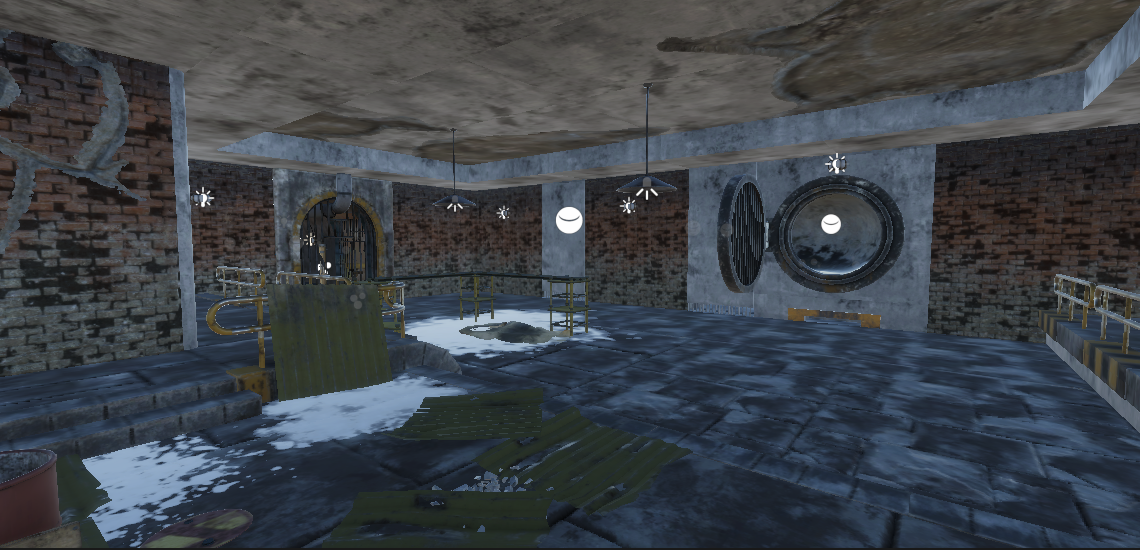
\includegraphics[width=.8\linewidth]{img/egouts/1.PNG}
  \captionof{figure}{\emph{Chapitre 3 - Les égouts}}
  \label{fig:chap3}
\end{minipage}%
\begin{minipage}{.5\textwidth}
  \centering
  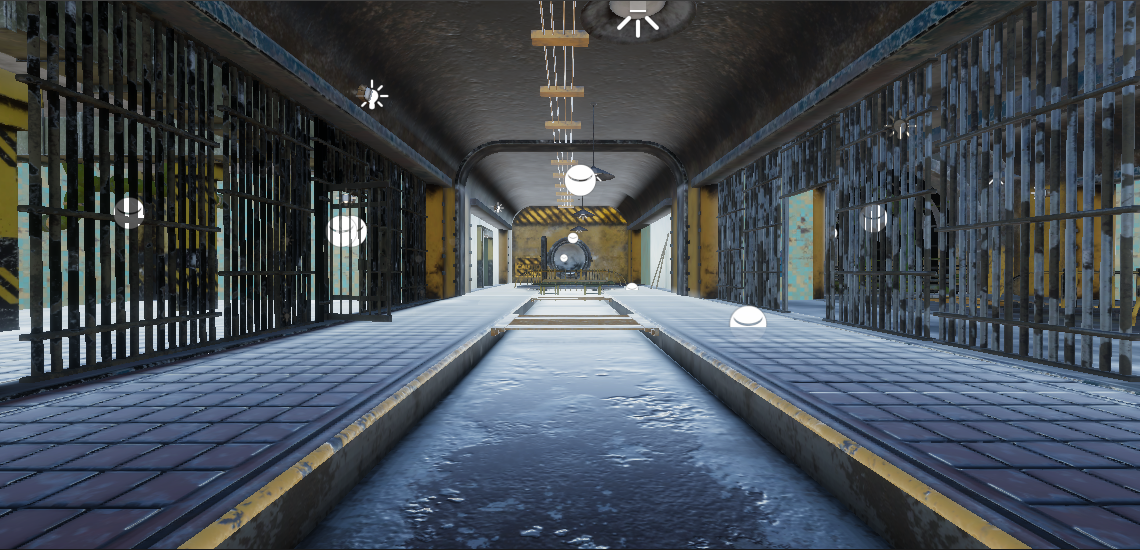
\includegraphics[width=.8\linewidth]{img/egouts/3.png}
  \captionof{figure}{\emph{Chapitre 3 - Les égouts}}
  \label{fig:chap3bis}
\end{minipage}
\end{figure}

\begin{figure}[H]
\centering
\begin{minipage}{.5\textwidth}
  \centering
  \centerline{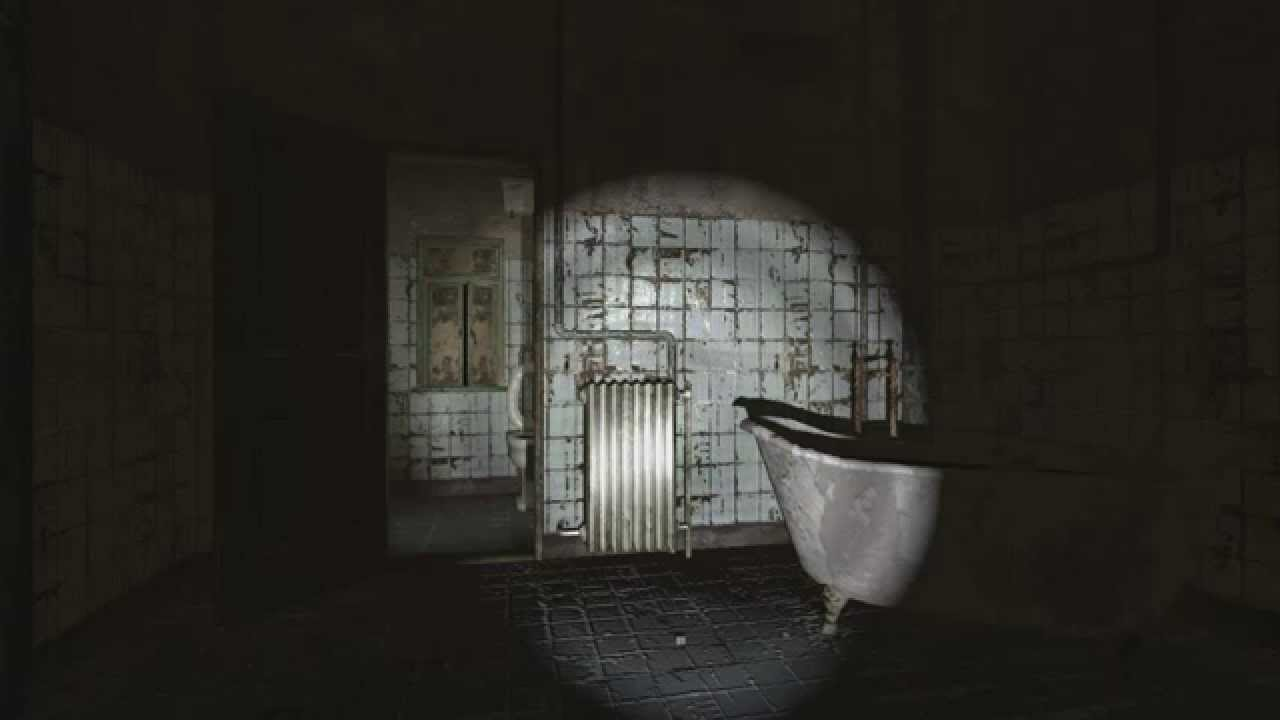
\includegraphics[width=1\linewidth]{img/egouts/light.jpg}}
  \captionof{figure}{\emph{Système de lampe torche}}
  \label{fig:flashlight}
\end{minipage}%
\end{figure}

Concernant les personnages jouables, nous comptons actuellement avec deux modèles de personnages complètement animés, un homme et une femme, provenant de la bibliothèque d’Adobe \emph{Mixamo}.
\newline

\begin{figure}[H]
\centering
\begin{minipage}{.5\textwidth}
  \centering
  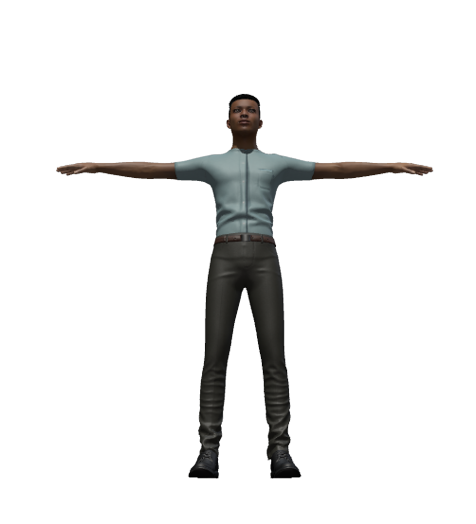
\includegraphics[width=.6\linewidth]{img/assets/remi.png}
  \captionof{figure}{\emph{Personnage masculin}}
  \label{fig:rémi}
\end{minipage}%
\begin{minipage}{.5\textwidth}
  \centering
  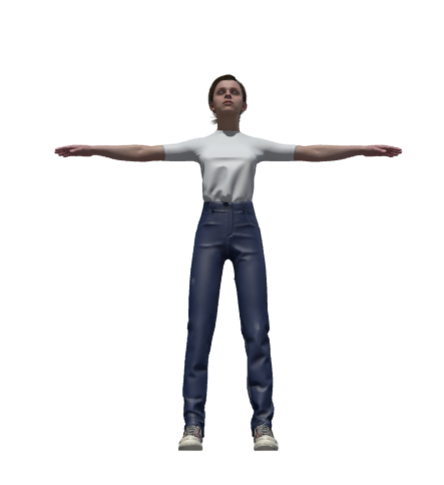
\includegraphics[width=.6\linewidth]{img/assets/sonia.png}
  \captionof{figure}{\emph{Personnage féminin}}
  \label{fig:sonia}
\end{minipage}
\end{figure}

Pour l'entité qui suivra le joueur plus tard dans le jeu, un modèle a déjà été choisi. (c.f. I.A. - Intelligence Artificielle)x
\vfill
\noindent\makebox[\linewidth]{\rule{.8\paperwidth}{.6pt}}\\[0.2cm]
EPITA Toulouse - Projet S2 - 2022 \hfill Nyctalopia - gameHUB
\noindent\makebox[\linewidth]{\rule{.8\paperwidth}{.6pt}}
\newpage



\subsection{Multijoueur}
\setlength{\parindent}{5ex}
Pour le multijoueur nous avons décidé d'utiliser le SDK Steamworks fourni par Steam Inc. N'étant pas pas nativement compatible avec C\#, nous avons dû utiliser une bibliothèque tierce nommée {\emph{Steamworks.NET}}. Ce SDK permettra de créer des lobbys et d'intégrer une liste d'amis, qui facilitera la communication entre les deux joueurs étant donné que Steam est la plateforme de vente de jeux vidéos la plus populaire au monde avec 100+ millions de connexions mensuelles.

Avec tout ces outils en place, il nous a suffi de lire la documentation officielle de Steam, et de mettre en place un script consistant à créer et à joindre des lobbys grâces aux boutons présents au sein de l'interface (c.f. UI/UX).

Pour la deuxième soutenance, nous avons décidé d'implémenter un chat vocal à l'aide de SteamVoice, fourni par Steam.

\vfill
\noindent\makebox[\linewidth]{\rule{.8\paperwidth}{.6pt}}\\[0.2cm]
EPITA Toulouse - Projet S2 - 2022 \hfill Nyctalopia - gameHUB
\noindent\makebox[\linewidth]{\rule{.8\paperwidth}{.6pt}}
\newpage

\subsection{UI/UX - Interface}
\setlength{\parindent}{5ex}
L'interface utilisateur possède trois parties principales, le menu principal, le menu ``Play'' et le menu ``Paramètres''. Ce dernier permet à l'utilisateur de pouvoir régler la résolution, la taille de la fenêtre (fenêtré, borderless ou plein écran), mais également le son et le choix des touches (AZERTY ou QWERTY).
Le menu ``Play'' possède trois boutons, un placé à gauche, permettant au joueur 1 de créer un lobby et de le rejoindre, et à droite deux boutons permettent au joueur 2 de soit, joindre le lobby avec un \emph{CSteamID} (code de lobby délivré par Steam) ou bien en utilisant sa liste d'ami Steam.
Enfin, le menu principal possède deux grands boutons appelant le joueur à soit débuter une nouvelle campagne ou bien de continuer là où il avait sauvegardé pour la dernière fois (c.f. Sauvegardes)

\begin{figure}[H]
\centering
\begin{minipage}{.5\textwidth}
  \centering
  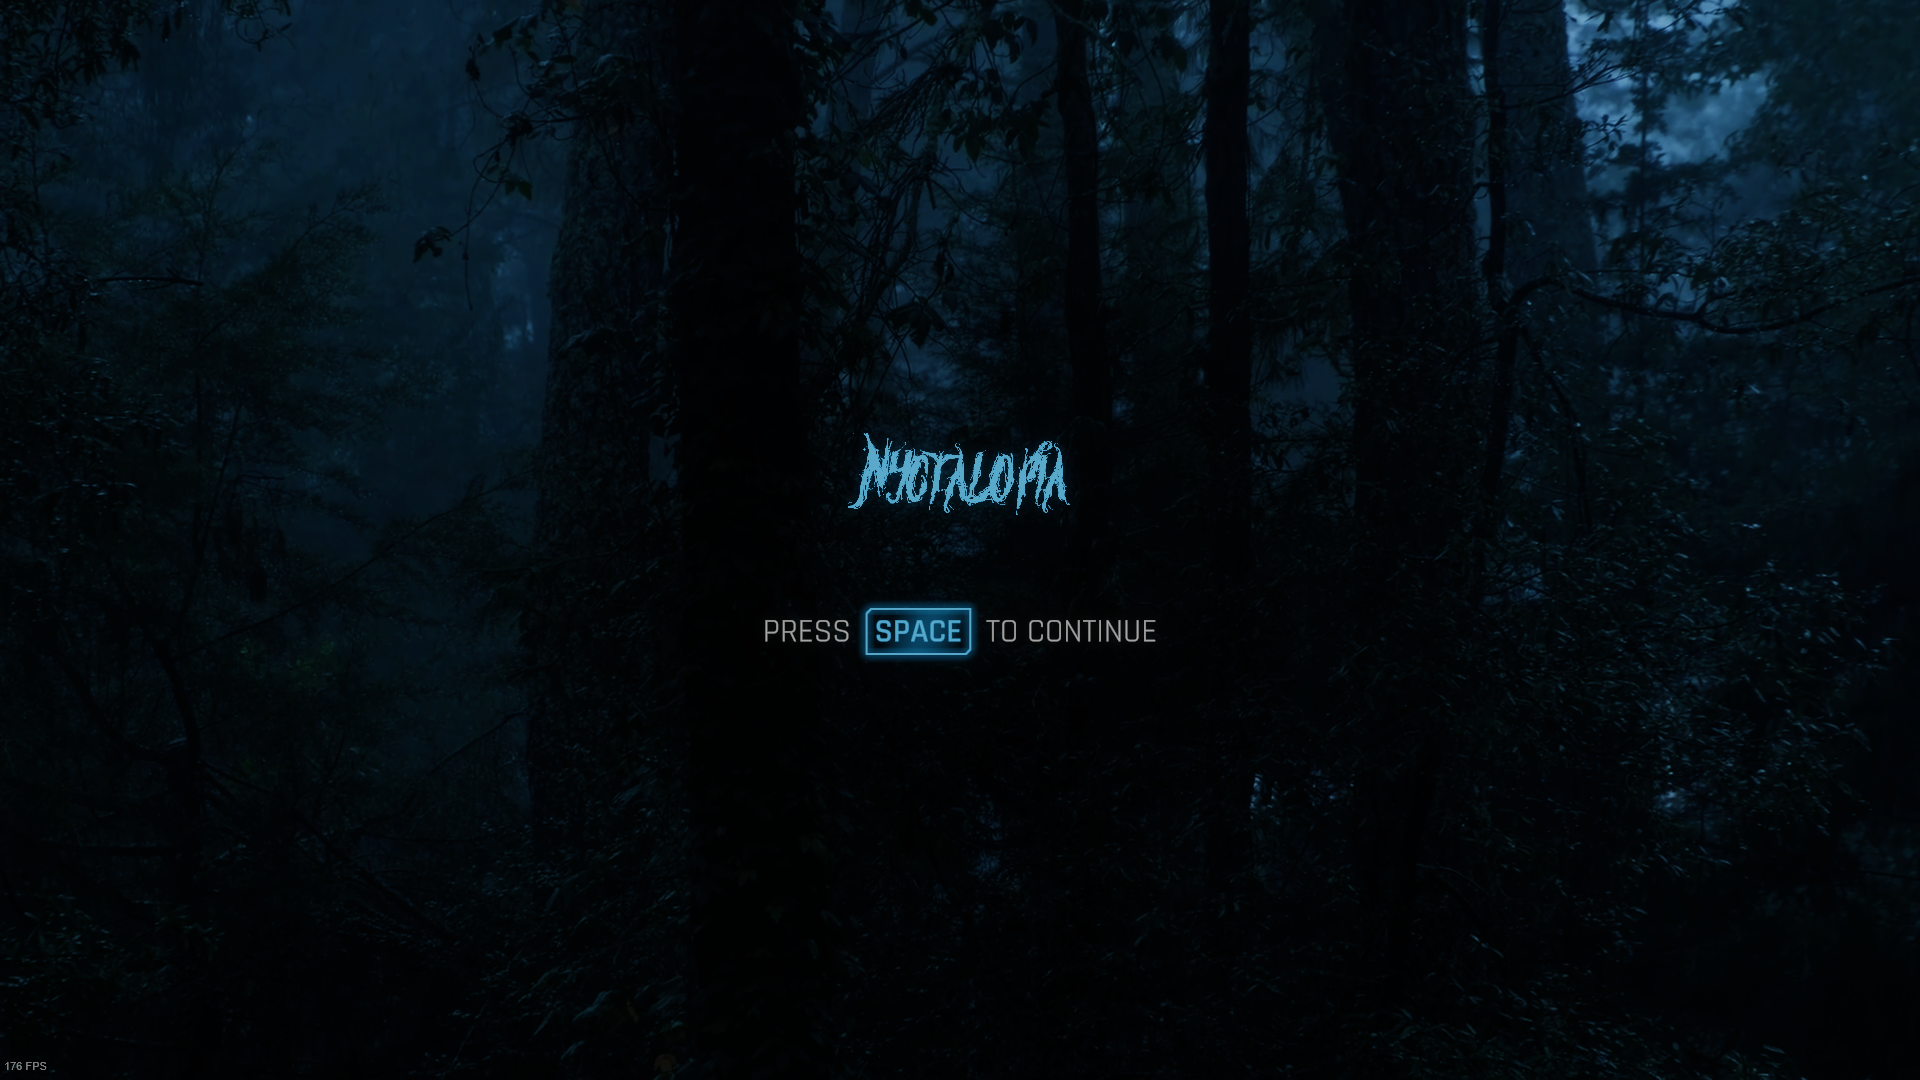
\includegraphics[width=.9\linewidth]{img/ui/UI2.png}
  \captionof{figure}{\emph{Écran d'accueil}}
  \label{fig:uihome}
\end{minipage}%
\begin{minipage}{.5\textwidth}
  \centering
  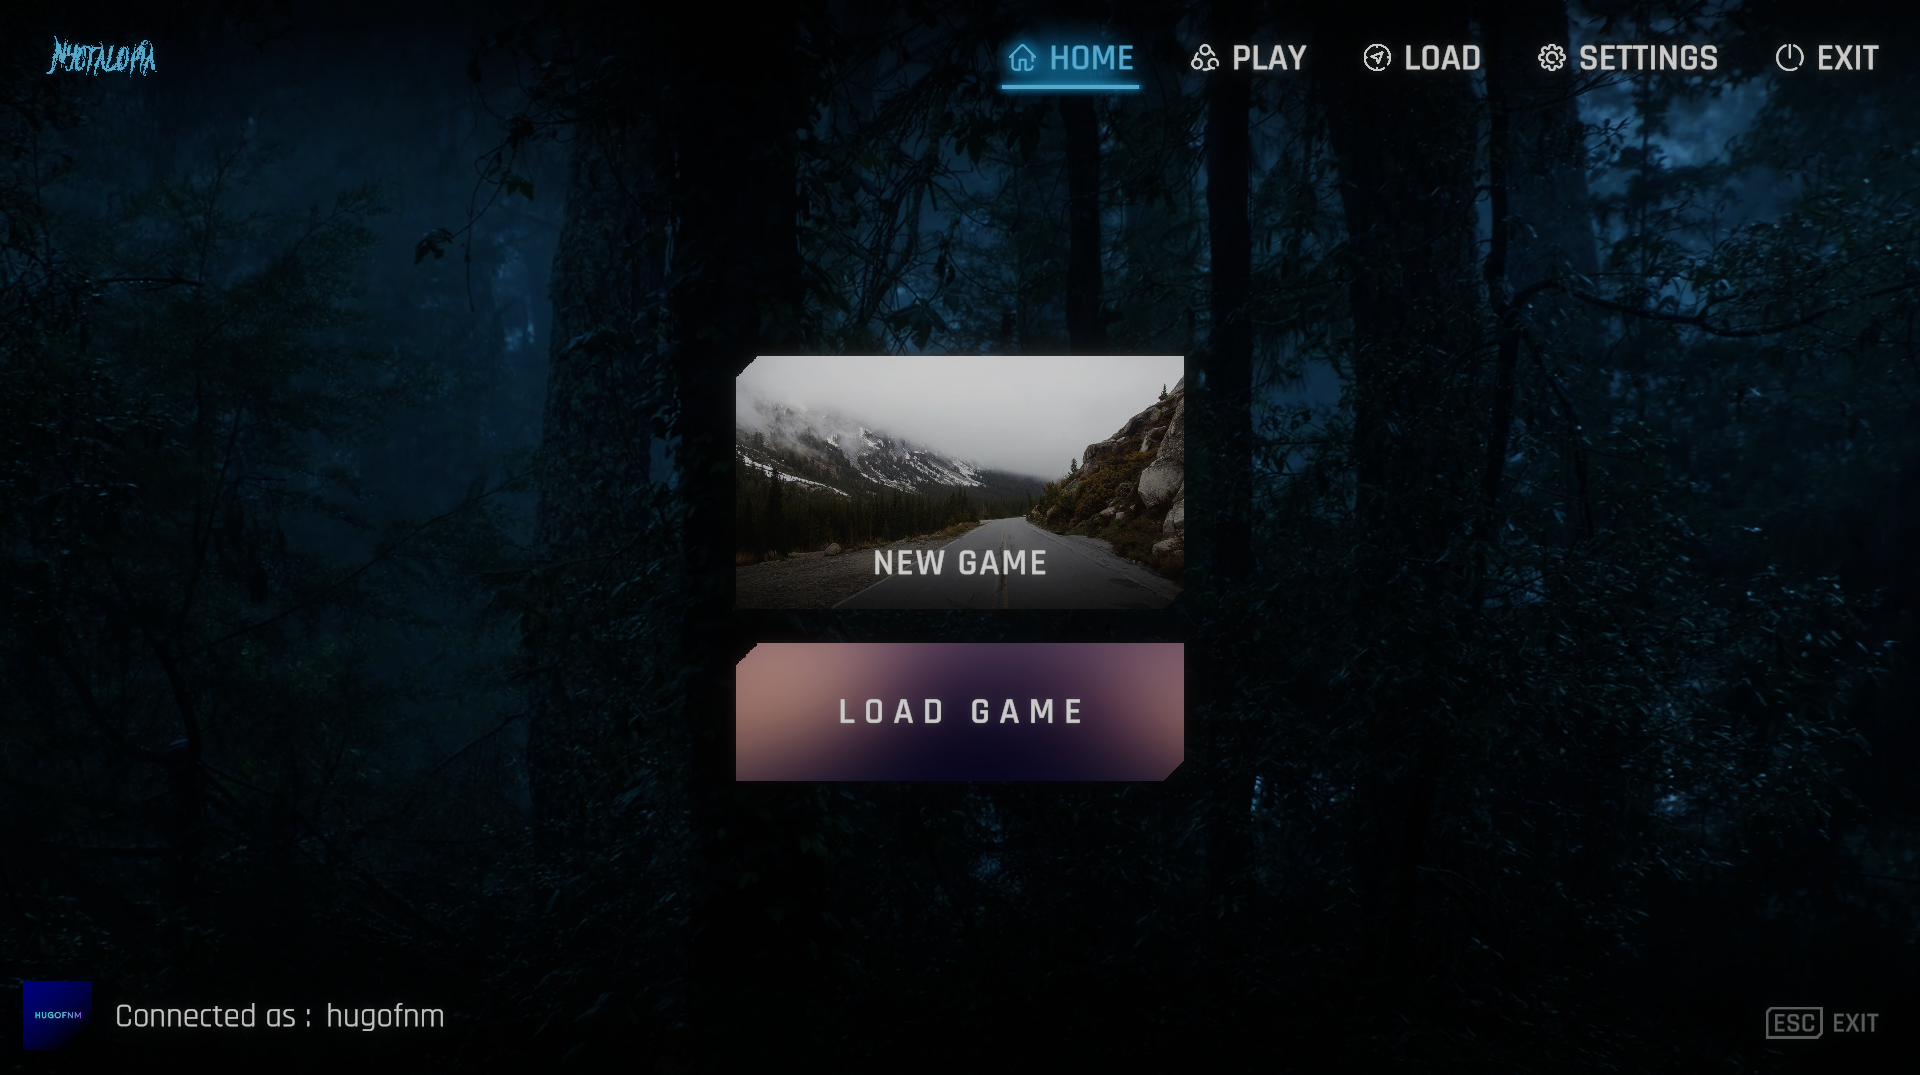
\includegraphics[width=.9\linewidth]{img/ui/UI1.png}
  \captionof{figure}{\emph{Menu principal}}
  \label{fig:uihome2}
\end{minipage}
\end{figure}

\begin{figure}[H]
\centering
\begin{minipage}{.5\textwidth}
  \centering
  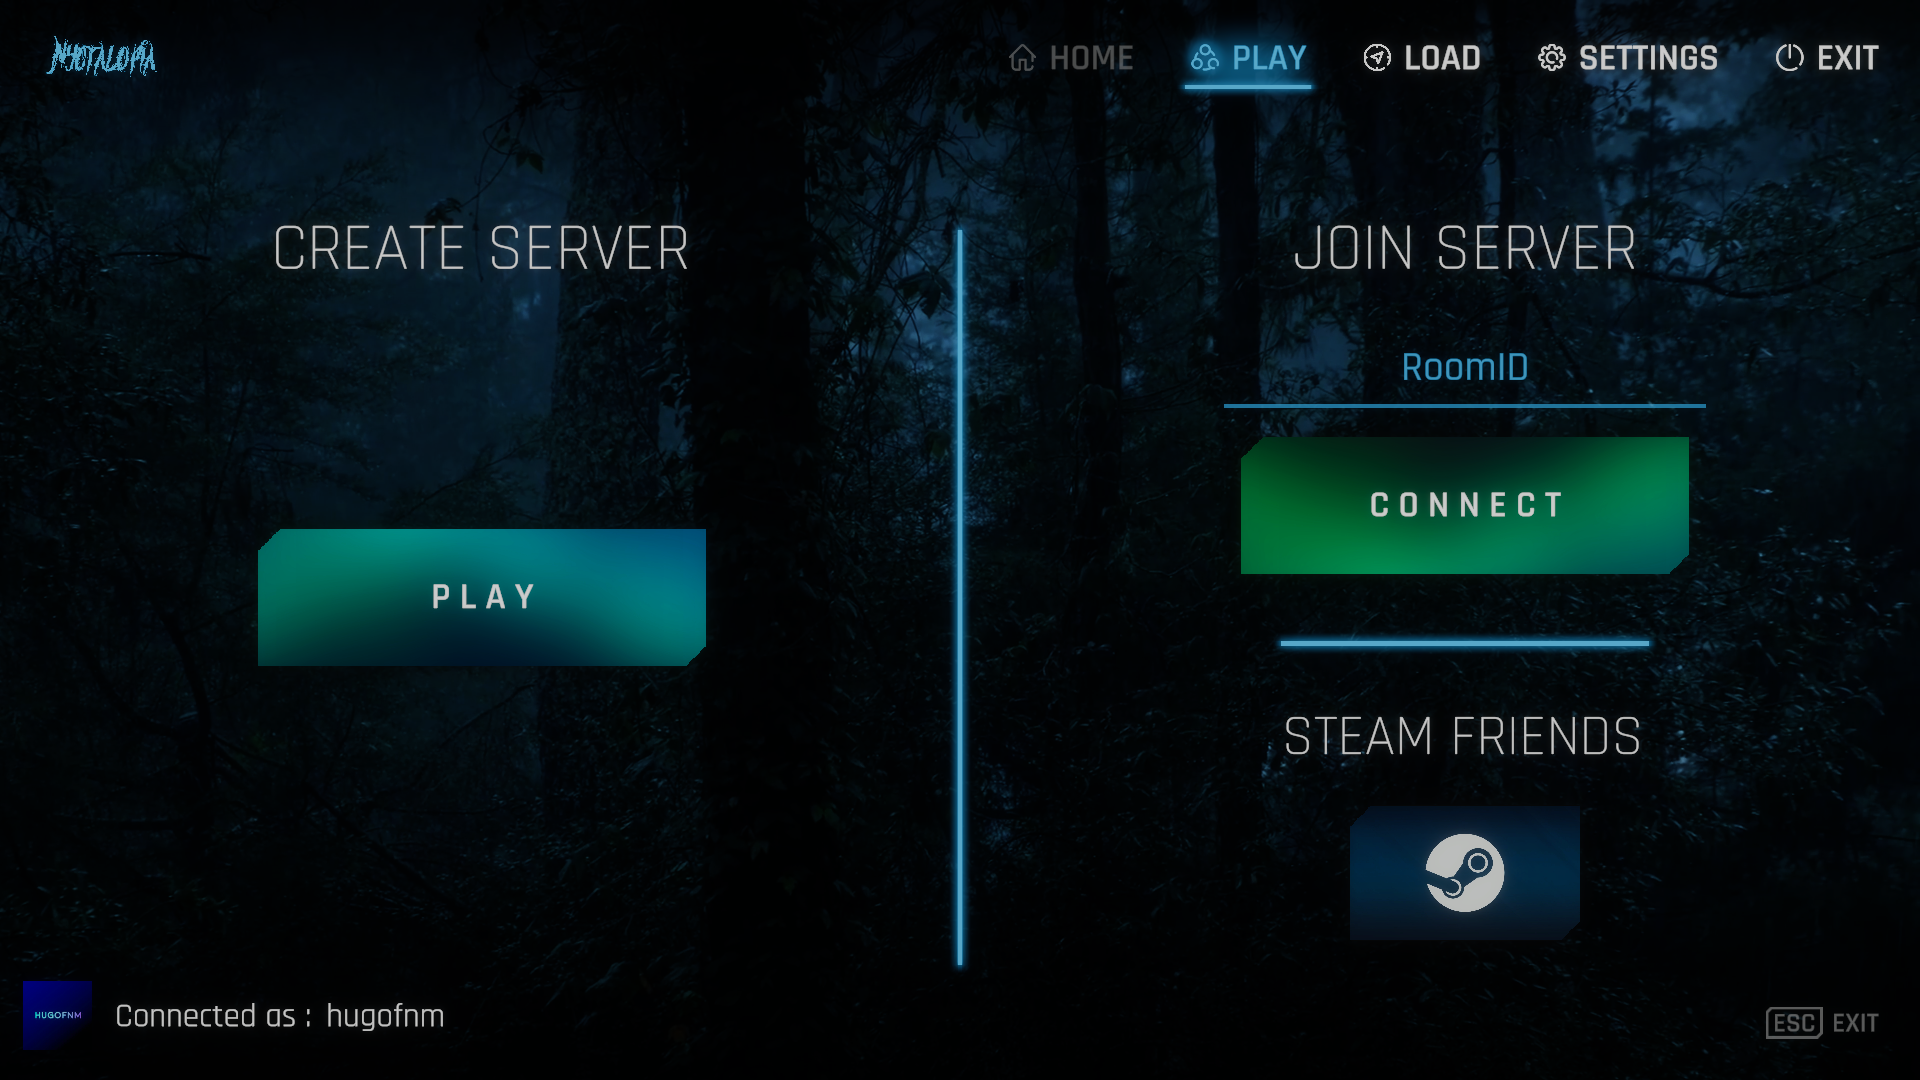
\includegraphics[width=.9\linewidth]{img/ui/UI.png}
  \captionof{figure}{\emph{Menu ``Play''}}
  \label{fig:uiplay}
\end{minipage}%
\begin{minipage}{.5\textwidth}
  \centering
  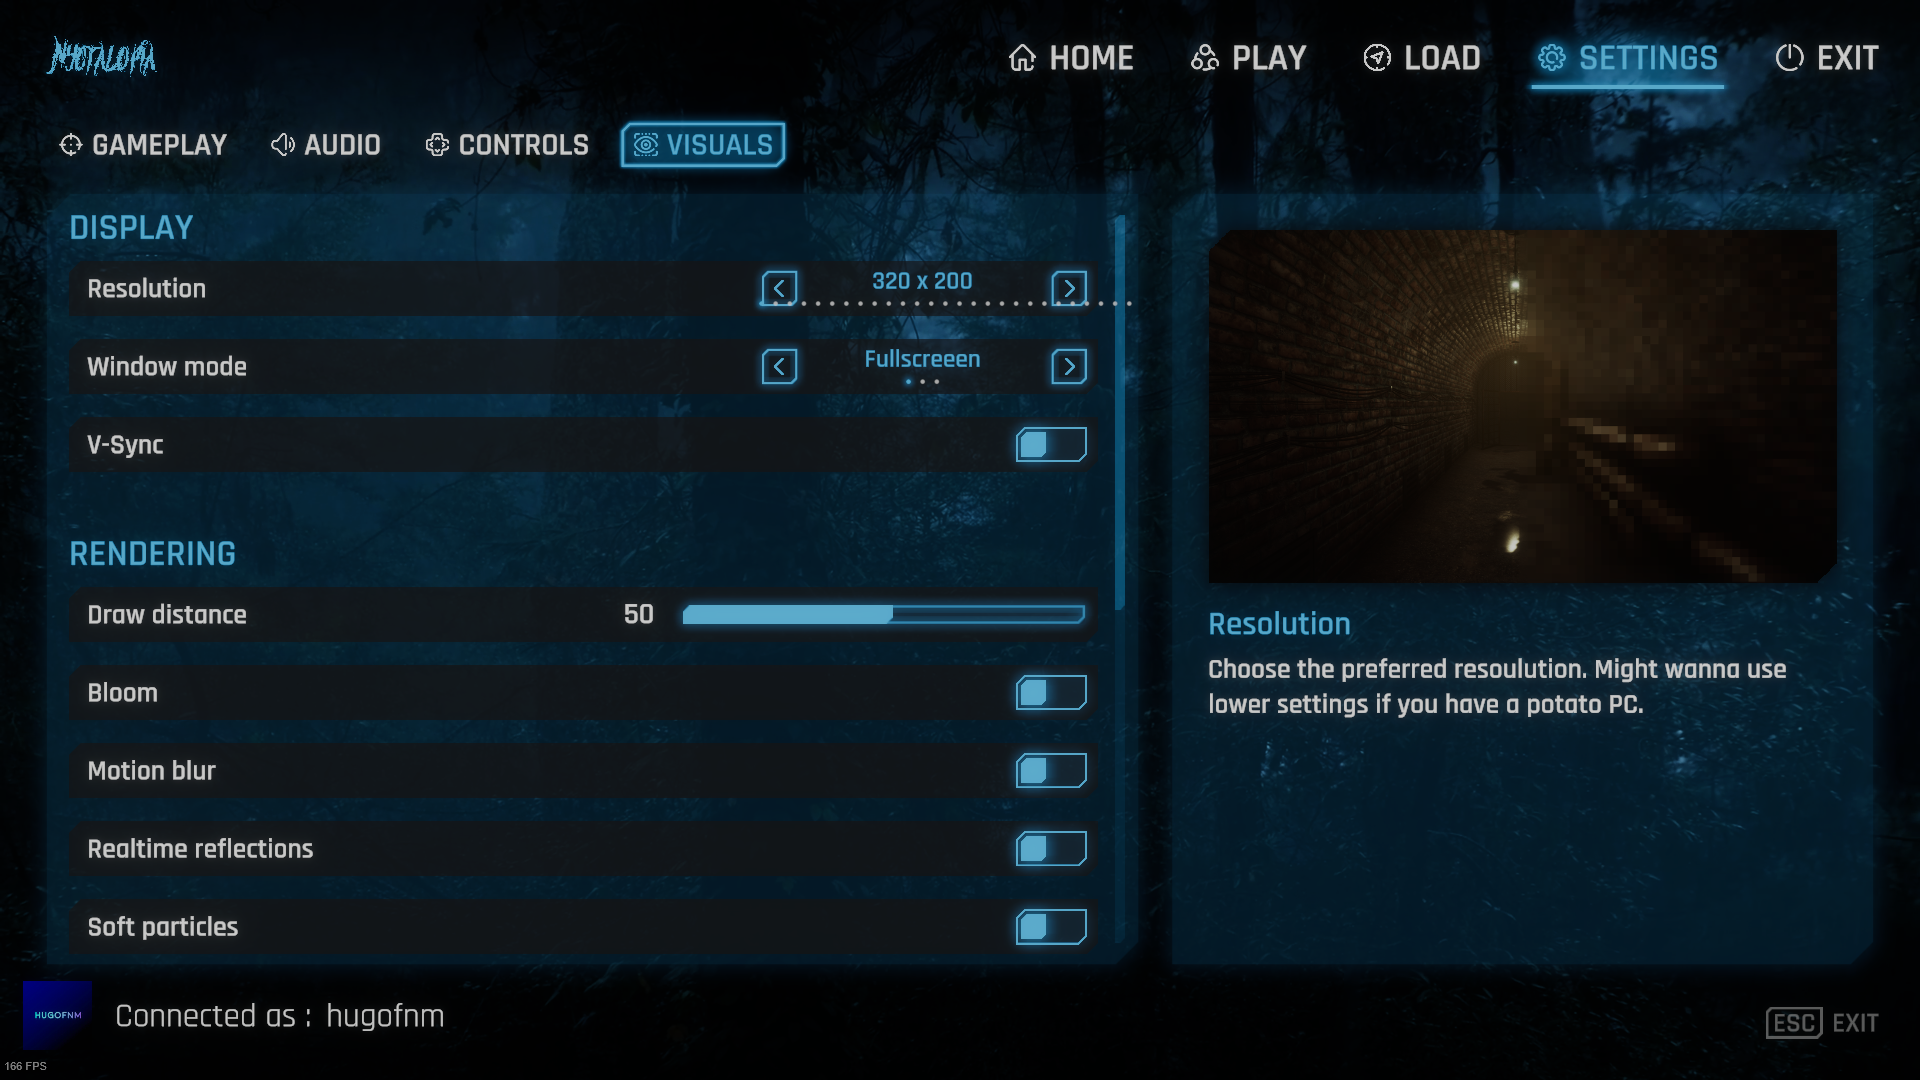
\includegraphics[width=.9\linewidth]{img/ui/UI4.png}
  \captionof{figure}{\emph{Menu ``Paramètres''}}
  \label{fig:uisettings}
\end{minipage}
\end{figure}

Il est désormais possible aussi de changer la langue du jeu. Trois options sont possibles : français, anglais ou espagnol.

\begin{figure}[H]
\centering
\begin{minipage}{.5\textwidth}
  \centering
  \centerline{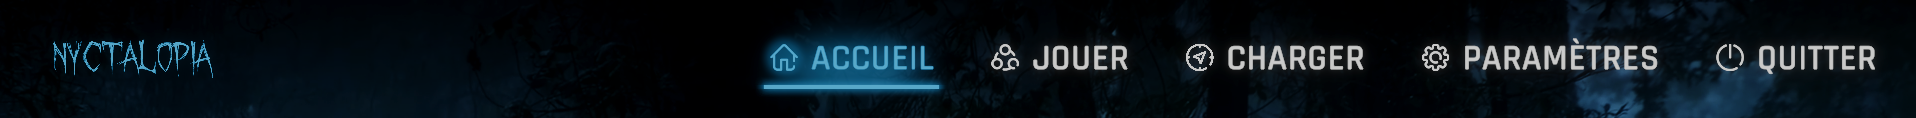
\includegraphics[width=2\linewidth]{img/uwufolder/fr.png}}
  \captionof{figure}{\emph{Français}}
  \label{fig:fr}
\end{minipage}%
\end{figure}

\vfill
\noindent\makebox[\linewidth]{\rule{.8\paperwidth}{.6pt}}\\[0.2cm]
EPITA Toulouse - Projet S2 - 2022 \hfill Nyctalopia - gameHUB
\noindent\makebox[\linewidth]{\rule{.8\paperwidth}{.6pt}}

\begin{figure}[H]
\centering
\begin{minipage}{.5\textwidth}
  \centering
  \centerline{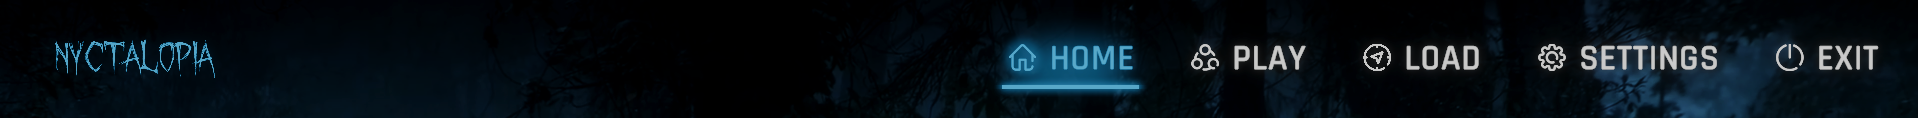
\includegraphics[width=2\linewidth]{img/uwufolder/en.png}}
  \captionof{figure}{\emph{Anglais}}
  \label{fig:en}
\end{minipage}%
\end{figure}

\begin{figure}[H]
\centering
\begin{minipage}{.5\textwidth}
  \centering
  \centerline{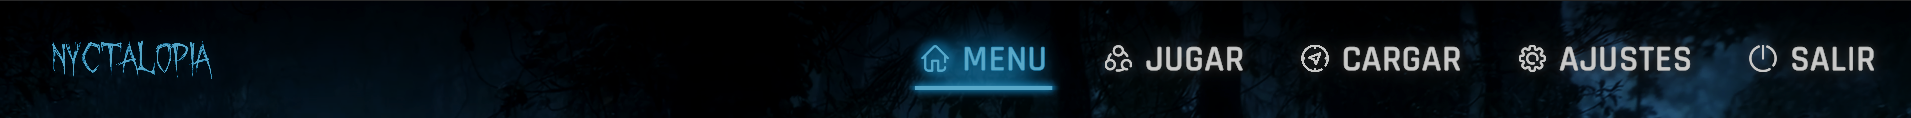
\includegraphics[width=2\linewidth]{img/uwufolder/es.png}}
  \captionof{figure}{\emph{Espagnol}}
  \label{fig:es}
\end{minipage}%
\end{figure}

Si l'utilisateur n'a pas effectué de choix, la langue par défaut sera réglée par rapport à la langue système (le système d'exploitation envoie au jeu la langue principale du système).

\begin{figure}[H]
\centering
\begin{minipage}{.5\textwidth}
  \centering
  \centerline{
\includegraphics[width=1\linewidth]{img/uwufolder/selector.png}}
  \captionof{figure}{\emph{Sélection de la langue dans le menu Paramètres}}
  \label{fig:languageselector}
\end{minipage}%
\end{figure}

Nous avons également mis en place un installateur graphique \emph{``.exe''} qui est accessible à tout utilisateur possédant une machine Windows ou Linux 64 Bits sur le site \emph{get.nyctalopia.games} (c.f Site Web). Ainsi qu'un script permettant d'informer ses amis que l'on joue à Nyctalopia sur la plateforme Discord a été créé.

\begin{figure}[H]
\centering
\begin{minipage}{.5\textwidth}
  \centering
  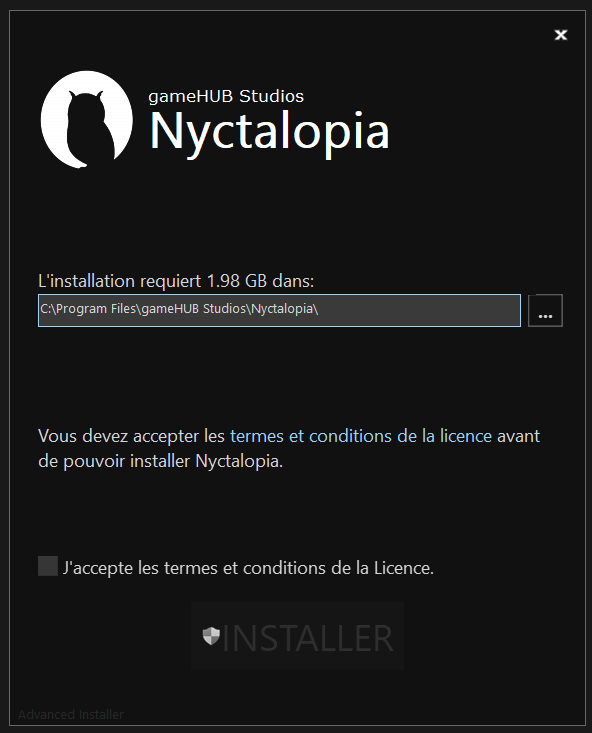
\includegraphics[width=.7\linewidth]{img/ui/installer.png}
  \captionof{figure}{\emph{Installateur Graphique \emph{.exe}}}
  \label{fig:uiinstall}
\end{minipage}%
\begin{minipage}{.5\textwidth}
  \centering
  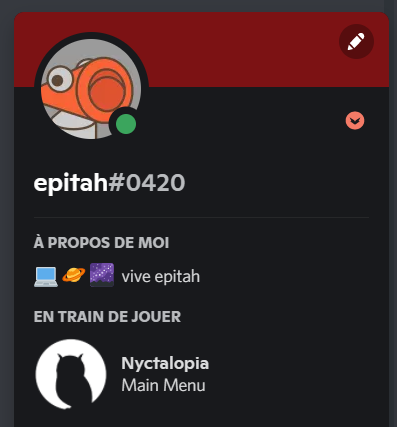
\includegraphics[width=.9\linewidth]{img/ui/DRPC.png}
  \captionof{figure}{\emph{Discord Rich Presence}}
  \label{fig:drpc}
\end{minipage}
\end{figure}

\vfill
\noindent\makebox[\linewidth]{\rule{.8\paperwidth}{.6pt}}\\[0.2cm]
EPITA Toulouse - Projet S2 - 2022 \hfill Nyctalopia - gameHUB
\noindent\makebox[\linewidth]{\rule{.8\paperwidth}{.6pt}}
\newpage

\subsection{Manuels d'instructions et d'installation}
\setlength{\parindent}{5ex}
Pour la deuxième soutenance nos manuels d'instructions et d'installation sont entièrement complets et vont permettre aux utilisateurs qui rencontreront des problèmes d'avoir tout de suite des réponses à leurs questions. On y retrouve une version en français mais aussi en anglais.  

\begin{figure}[H]
\centering
\begin{minipage}{.5\textwidth}
  \centering
  \centerline{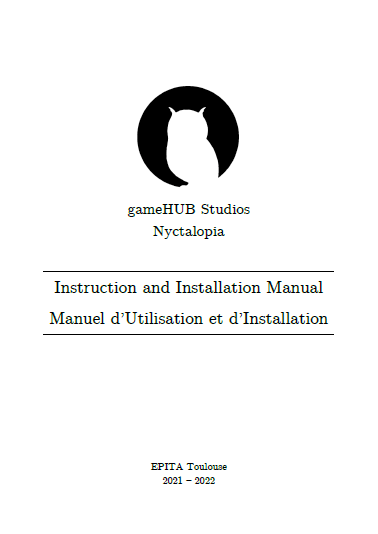
\includegraphics[width=0.8\linewidth]{img/M1.png}}
  \captionof{figure}{\emph{Première page}}
  \label{fig:manual}
\end{minipage}%
\end{figure}


\subsection{Site Web}
\setlength{\parindent}{5ex}
Pour cette deuxième soutenance, nous avons décidé d'achever notre site web, qui est prêt au public. 

Nous avons essayé de rendre le site attractif. On peut le voir avec les effets qui permettent que l'arrière-plan et les images au premier plan ne défile pas à la même vitesse ou encore avec le curseur qui suit la souris.
Pour ces effets, on a fait le choix d'utiliser des scripts JS fournis par Internet pour se rapprocher le plus possible d'un vrai site professionnel. Le code HTML est très bien organisé pour nous permettre d'améliorer ou de modifier le site à tout moment. 

\vfill
\noindent\makebox[\linewidth]{\rule{.8\paperwidth}{.6pt}}\\[0.2cm]
EPITA Toulouse - Projet S2 - 2022 \hfill Nyctalopia - gameHUB
\noindent\makebox[\linewidth]{\rule{.8\paperwidth}{.6pt}}
\newpage

Nous avons choisi un fond sombre pour tout de suite mettre le joueur dans l'ambiance du jeu où il sera dans l'obscurité. Enfin, le site est adapté pour tout type d'écrans ce qui permet au joueur de nous consulter n'importe quand. A travers ce site nous voulons mettre en confiance l'utilisateur et lui donner envie de jouer en montrant des informations intéressantes sur Nyctalopia et en montrant notre professionnalisme.
 
Pour cette soutenance nous avons apporté quelques modifications à notre site pour le rendre plus agréable à parcourir et à utiliser. 

\noindent En terme de contenu sur le site on peut retrouver:
\begin{itemize}
    \item Une page d'accueil : forêt animée
    
\begin{figure}[H]
\centering
\begin{minipage}{.5\textwidth}
  \centering
  \centerline{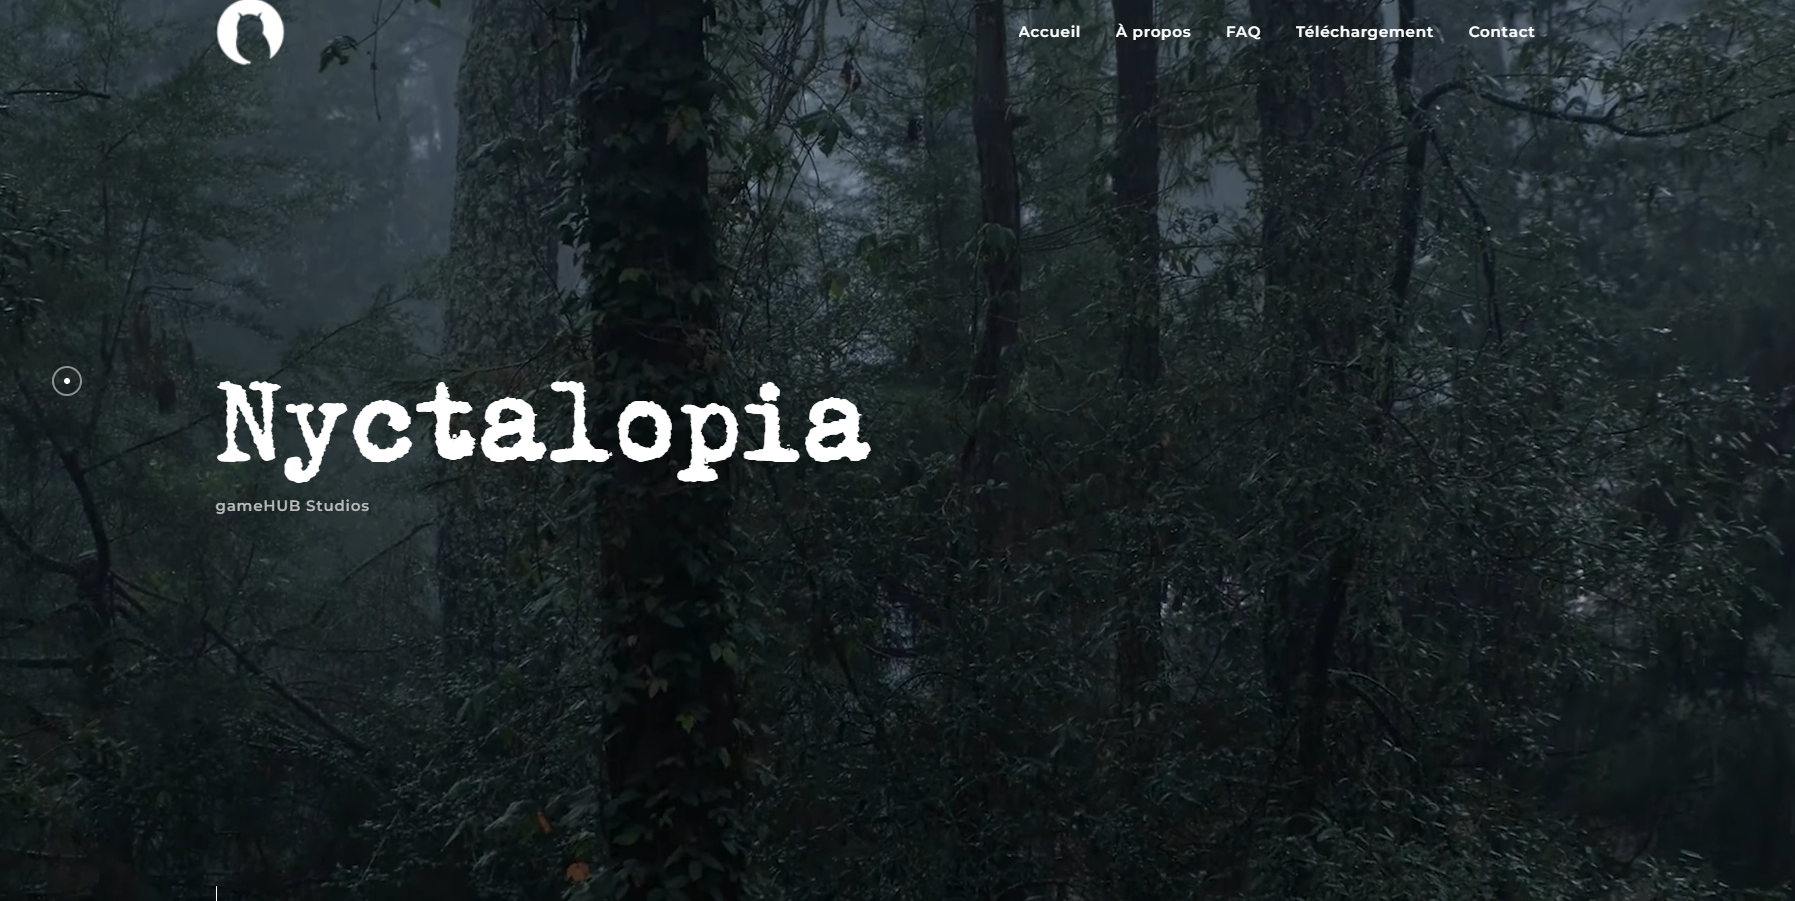
\includegraphics[width=1\linewidth]{img/acceuil.PNG}}
  \captionof{figure}{\emph{Accueil du site}}
  \label{fig:accueil}
\end{minipage}%
\end{figure}    
    
    \item Image du jeu: tels que la forêt ou encore l'interface utilisateur mais également la scène d'introduction
    
\begin{figure}[H]
\centering
\begin{minipage}{.5\textwidth}
  \centering
  \centerline{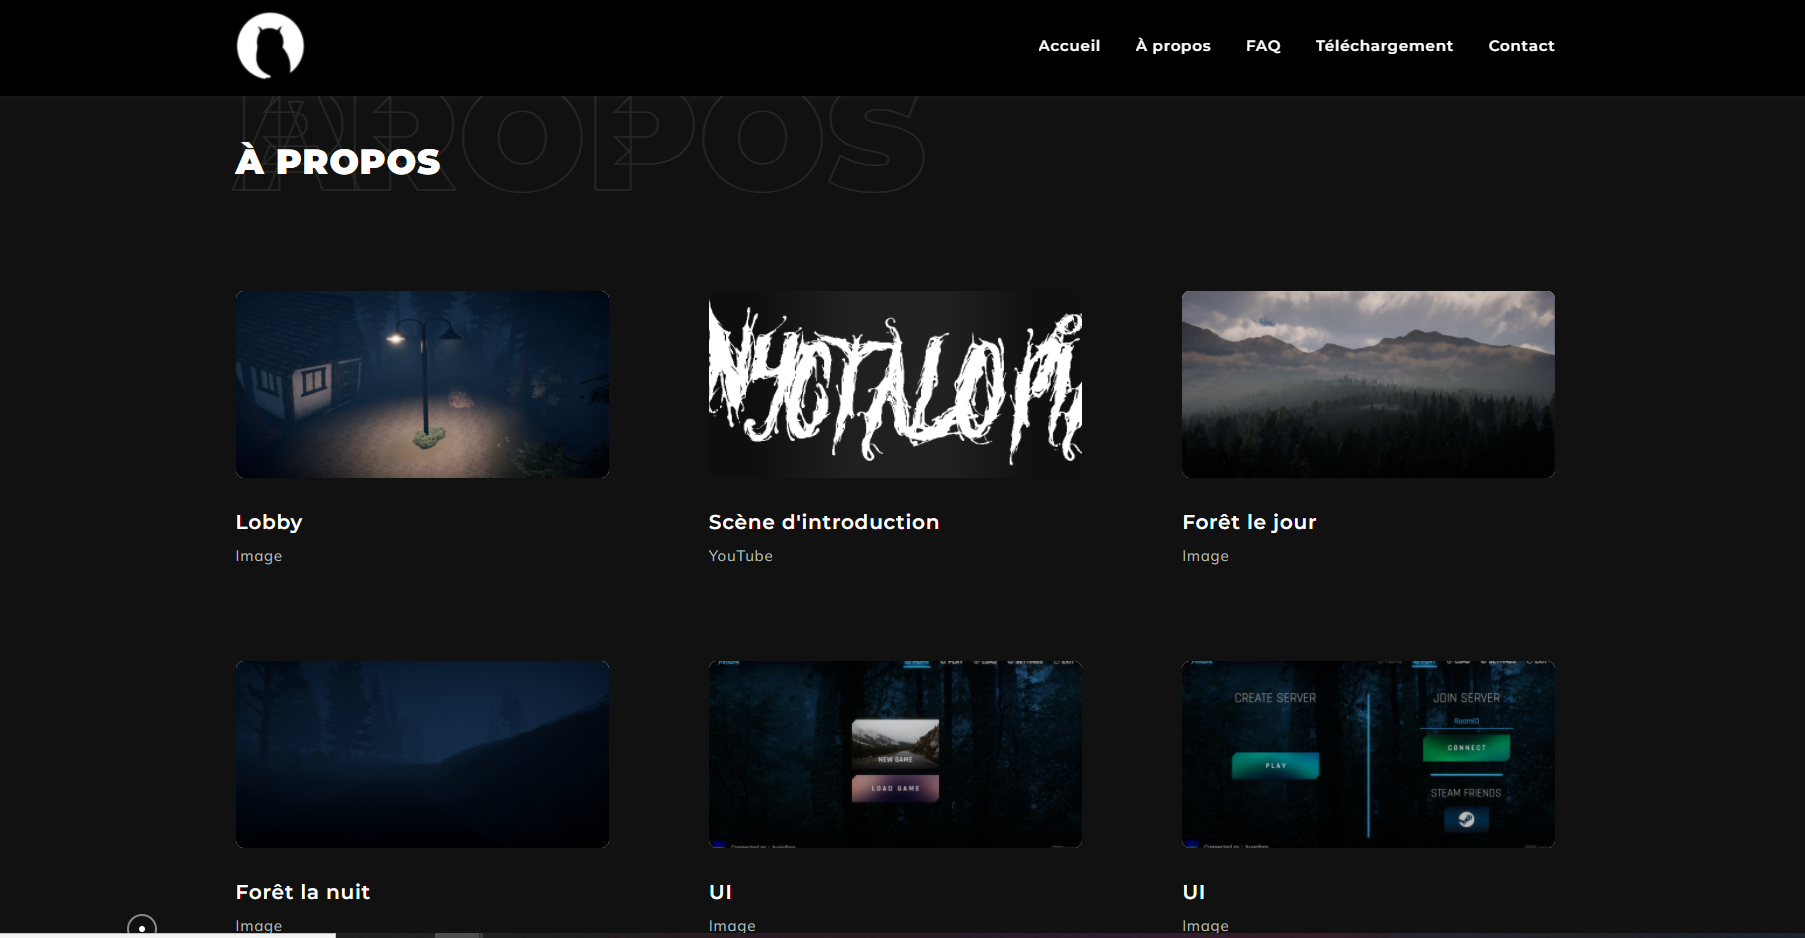
\includegraphics[width=1\linewidth]{img/propos.PNG}}
  \captionof{figure}{\emph{Image du jeu}}
  \label{fig:imggame}
\end{minipage}%
\end{figure}

\end{itemize}

\vfill
\noindent\makebox[\linewidth]{\rule{.8\paperwidth}{.6pt}}\\[0.2cm]
EPITA Toulouse - Projet S2 - 2022 \hfill Nyctalopia - gameHUB
\noindent\makebox[\linewidth]{\rule{.8\paperwidth}{.6pt}}
\newpage

\begin{itemize}

    \item Contact : Formulaire + courriel du studio : on peut retrouver maintenant un bouton "envoyer" qui nous renvoie vers notre boite mail. Pour l'instant il est inutile de remplir le formulaire mais pour la dernière soutenance nous implémenterons un script permettant de récupérer ce que l'utilisateur a écrit dans le formulaire pour le mettre directement dans un mail.
    
\begin{figure}[H]
\centering
\begin{minipage}{.5\textwidth}
  \centering
  \centerline{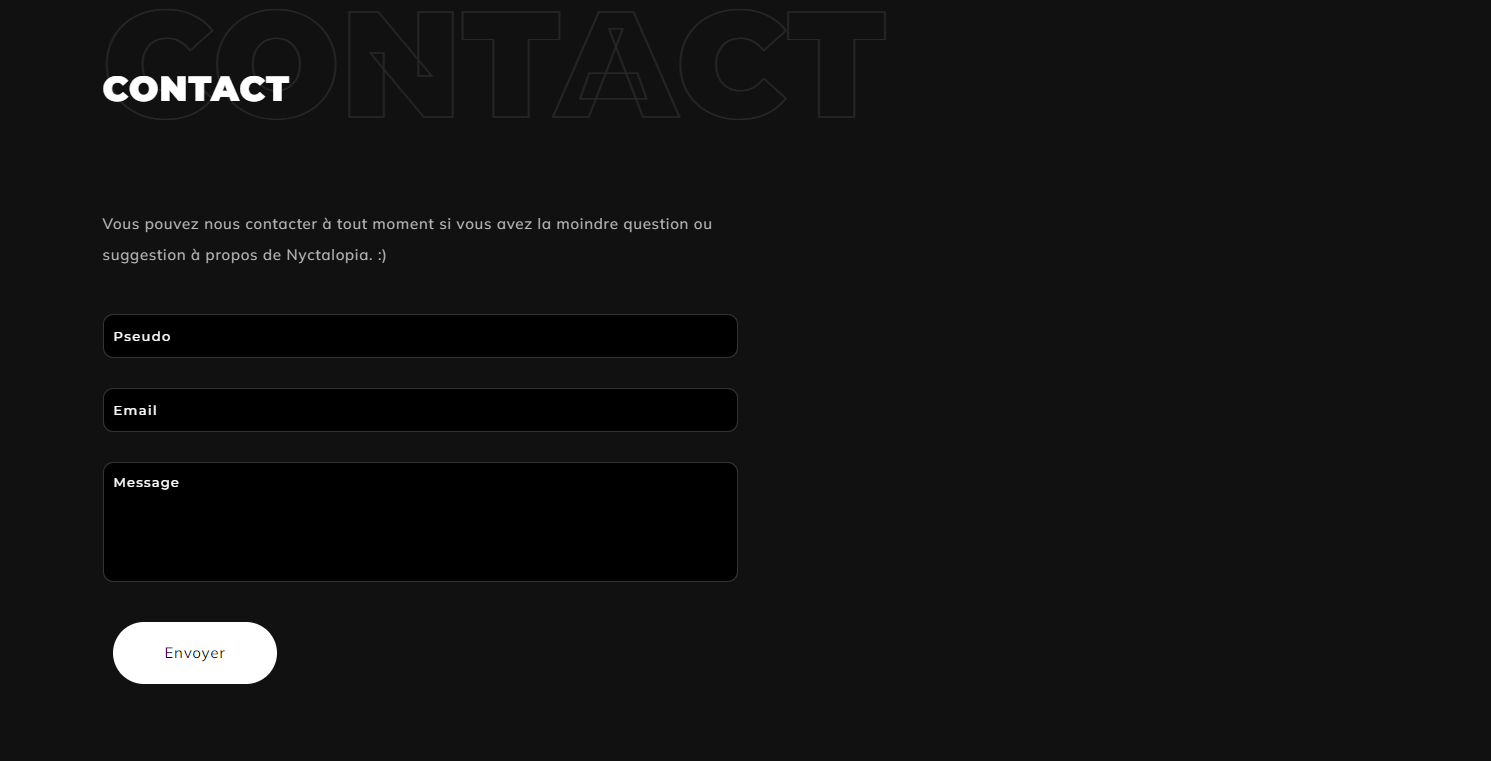
\includegraphics[width=1\linewidth]{img/Contact.png}}
  \captionof{figure}{\emph{Contact}}
  \label{fig:contact}
\end{minipage}%
\end{figure}


    \item Équipe: rôles de chaque membre 

\begin{figure}[H]
\centering
\begin{minipage}{.5\textwidth}
  \centering
  \centerline{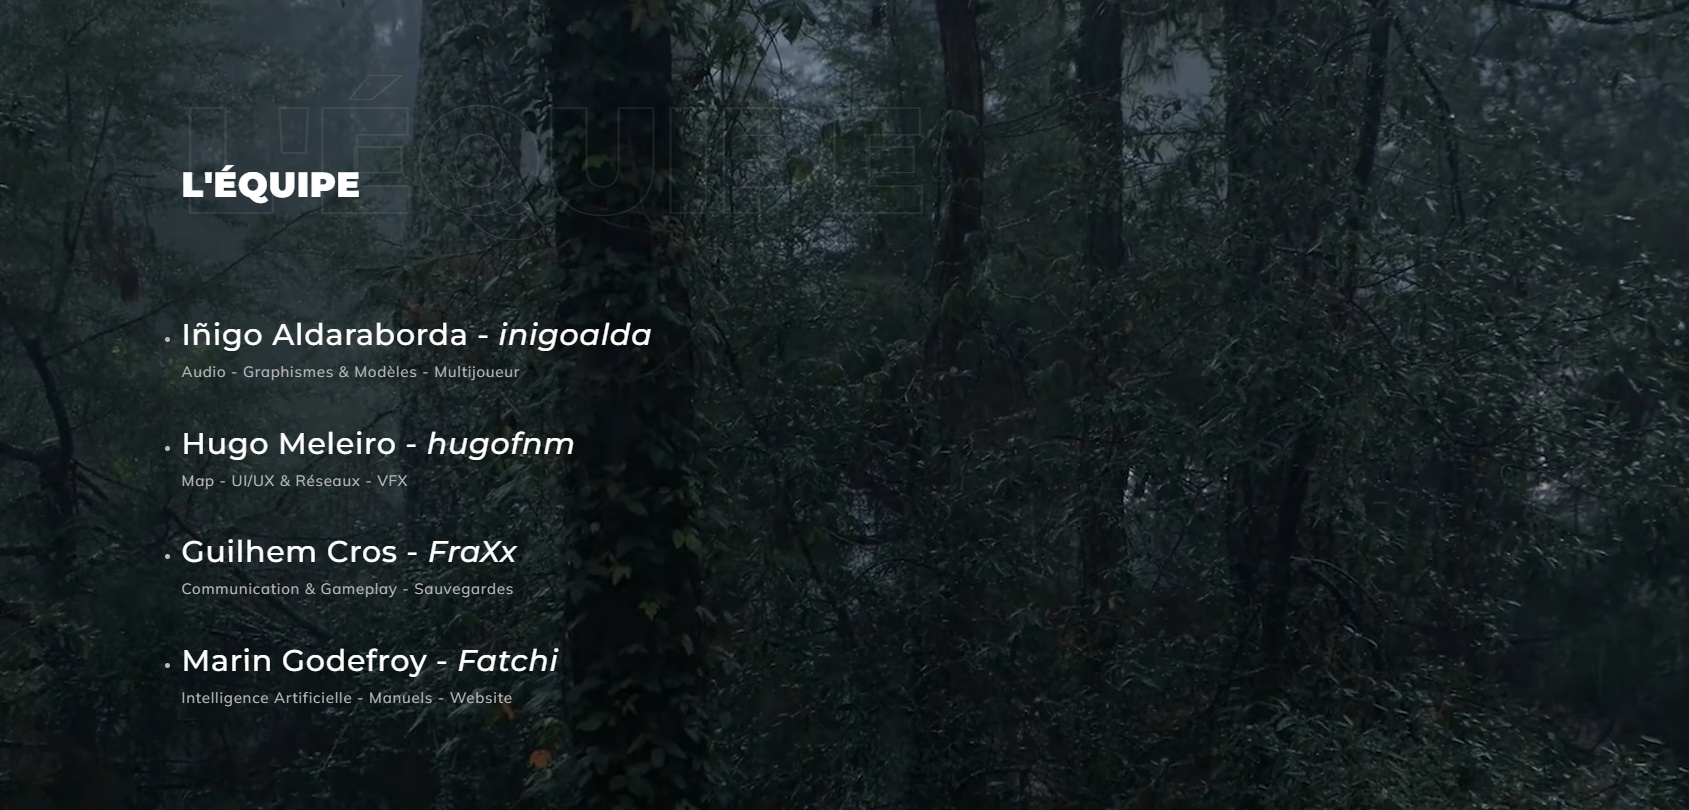
\includegraphics[width=1\linewidth]{img/team.PNG}}
  \captionof{figure}{\emph{Membres du studio GameHub}}
  \label{fig:team}
\end{minipage}%
\end{figure}
    

    \item FAQ: quelques réponses à des questions courantes.

\begin{figure}[H]
\centering
\begin{minipage}{.5\textwidth}
  \centering
  \centerline{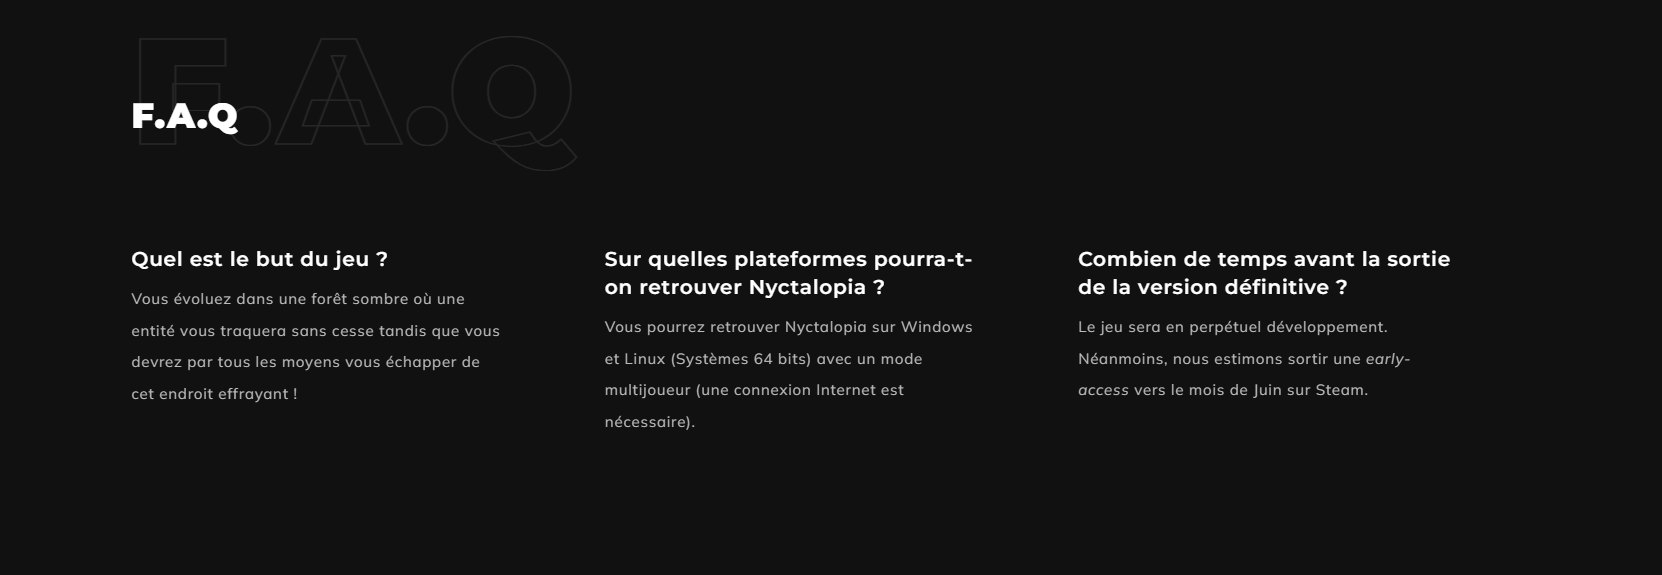
\includegraphics[width=1\linewidth]{img/faq.PNG}}
  \captionof{figure}{\emph{F.A.Q}}
  \label{fig:faq}
\end{minipage}%
\end{figure}

    \item Documents: Cahier des charges, rapport de soutenance

    \item Liens de téléchargements et Configurations : minimale et recommandée 

\end{itemize}

\vfill
\noindent\makebox[\linewidth]{\rule{.8\paperwidth}{.6pt}}\\[0.2cm]
EPITA Toulouse - Projet S2 - 2022 \hfill Nyctalopia - gameHUB
\noindent\makebox[\linewidth]{\rule{.8\paperwidth}{.6pt}}
\newpage


\begin{figure}[H]
\centering
\begin{minipage}{.5\textwidth}
  \centering
  \centerline{
\includegraphics[width=1.5\linewidth]{img/ssl.png}}
  \captionof{figure}{\emph{Site sécurisé SSL}}
  \label{fig:ssl}
\end{minipage}%
\end{figure}

Le site web est hébergé sur CloudFlare Pages, un service gratuit de l'entreprise de gestion DNS CloudFlare, permettant de déployer rapidement à partir d'un repo Git, un site web statique rapide grâce aux serveurs CDN disposés partout dans le monde et sécurisé par un certificat SSL et une protection anti-DDOS.
Le nom de domaine choisi est \emph{nyctalopia.games}. Il est simple et facile à retenir pour l'utilisateur.

\begin{figure}[H]
\centering
\begin{minipage}{.5\textwidth}
  \centering
  \centerline{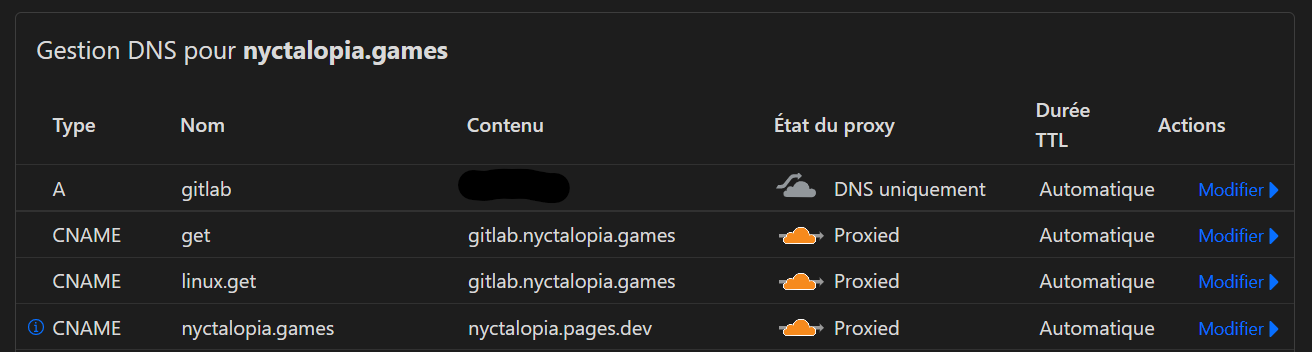
\includegraphics[width=2\linewidth]{img/ui/dns.png}}
  \captionof{figure}{\emph{Interface CloudFlare}}
  \label{fig:dns}
\end{minipage}%
\end{figure}

Nous avons également décidé de mettre en place un GitLab (\emph{gitlab.nyctalopia.games}) privé sur un serveur nous appartenant, ce qui nous a permis d'utiliser la puissance brute de Git LFS et des pipelines CI/CD, améliorant notre productivité sans perdre de temps.

\vfill
\noindent\makebox[\linewidth]{\rule{.8\paperwidth}{.6pt}}\\[0.2cm]
EPITA Toulouse - Projet S2 - 2022 \hfill Nyctalopia - gameHUB
\noindent\makebox[\linewidth]{\rule{.8\paperwidth}{.6pt}}

\newpage